% ==================== %
% == RESOURCES USED == %
% ==================== %


\begin{filecontents*}[overwrite]{gallery-showcase-bw.tex}
\documentclass[theme = bw]{tutodoc}

\usepackage{multicol}
\usepackage{lastpage}

\renewcommand*\pagemark{%
  \usekomafont{pagenumber}{\thepage\kern1pt/\kern1pt\pageref*{LastPage}}%
}


\newcommand\thisstyle{bw}


\newcommand\myexrmktext{
    \tdocversion{1.7.0}[2024-12-04]
    In the flow of the text, it is always useful to be able to provide examples and comments to supplement the main content.
}


\newcommand\myadmotext{
    Depending on the context of use, it is sometimes necessary to be able to highlight content by indicating its degree of importance.
}

\newcommand\myhighlightedtextnonote{
    What to say?
    I don't know, but it's nice. No ?
}

\newcommand\myhighlightedtext{
    What to say\,%
    \footnote{
        Let's not forget the footnotes...
    }?
    I don't know, but it's nice. No ?
}


\newcommand\mychgestext{
    In a change log, it is important to visualise the types of changes clearly. This makes it easier for the user to read!
}


\ExplSyntaxOn

\int_new:N \g__tutodoc_for_doc_int

\ExplSyntaxOff



\begin{document}

\textsf{\Huge\bfseries The \texttt{"\thisstyle"} theme}

\section{Liens}

{\Large\bfseries \href{https://github.com/bc-tools/for-latex/tree/main/tutodoc}{A very big link}}, but at least we can see it.



\section{\LaTeX\ listings}

Typing inline code such as \tdoclatexin{E = m c^2 \neq \pi \neq \frac{3}{14}} is useful, as is showing use cases such as the following one.

\begin{tdoclatex}
Formatted \LaTeX\ code is great: $E = m c^2$ or $pi \neq \frac{3}{14}$.
\end{tdoclatex}


There's also a less invasive side-by-side mode. Nice! No ?

\begin{tdoclatex}<\tdoctcb{sbs}>
Formatted \LaTeX\ code is great:       \\
$E = m c^2$ or $\pi \neq \frac{3}{14}$.
\end{tdoclatex}



\section{Highlighting, versioning and dating}

\subsection{tdocexa, tdocrem}

\myexrmktext

\ExplSyntaxOn

\seq_map_inline:Nn \g__tutodoc_focus_std_seq {
    \begin{tdoc#1}
        \myhighlightedtext
    \end{tdoc#1}
}

\ExplSyntaxOff



\subsection{tdocnote, tdoctip...}

\myadmotext

\ExplSyntaxOn

\int_set:Nn \g__tutodoc_for_doc_int { 0 }

\ifcsundef{g__tutodoc_focus_color_seq}{
    \prop_map_inline:Nn \g__tutodoc_focus_color_prop {
        \int_gincr:N \g__tutodoc_for_doc_int

        \begin{tdoc#1}
      	  	\int_compare:nTF
	    		{\g__tutodoc_for_doc_int = 1 }
	    		{ \myhighlightedtext }
	    		{ \myhighlightedtextnonote }
        \end{tdoc#1}
    }
} {
    \seq_map_inline:Nn \g__tutodoc_focus_color_seq {
        \int_gincr:N \g__tutodoc_for_doc_int

        \begin{tdoc#1}
      	  	\int_compare:nTF
	    		{\g__tutodoc_for_doc_int = 1 }
	    		{ \myhighlightedtext }
	    		{ \myhighlightedtextnonote }
        \end{tdoc#1}
    }
}

\ExplSyntaxOff



\subsection{tdocbreak, tdocfix...}

\tdocstartproj{A new demonstration section...}

\begin{tdoctodo}
	\item A gallery would be welcome...
\end{tdoctodo}

\ifcsundef{g__tutodoc_topic_change_seq}{
 	\medskip
}{}

\mychgestext

\ifcsundef{g__tutodoc_topic_change_seq}{
	\medskip
}{}

\ExplSyntaxOn

\int_set:Nn \g__tutodoc_for_doc_int { 0 }

\begin{tabular}{%
	@{\hskip 0pt}p{.26\linewidth}%
	*{3}{@{\hskip 7pt}p{.23\linewidth}}@{\hskip 0pt}%
}
	\ifcsundef{g__tutodoc_topic_change_seq}{
    	\prop_map_inline:Nn \g__tutodoc_topic_change_prop {
          	\int_gincr:N \g__tutodoc_for_doc_int

          	\vspace{-12pt}

    	  	\begin{tdoc#1}
           		\item Infos...
    	  	\end{tdoc#1}

    	  	\int_compare:nTF
    	    	{\g__tutodoc_for_doc_int = 4 }
    	    	{ \\ }
    	    	{ & }
    	}
	}{
    	\seq_map_inline:Nn \g__tutodoc_topic_change_seq {
          	\int_gincr:N \g__tutodoc_for_doc_int

          	\vspace{-5pt}

    	  	\begin{tdoc#1}
           		\item Infos...
    	  	\end{tdoc#1}

    	  	\int_compare:nTF
    	    	{\g__tutodoc_for_doc_int = 4 }
    	    	{ \\ }
    	    	{ & }
    	}
	}
\end{tabular}

\ExplSyntaxOff

\end{document}

\end{filecontents*}

\begin{filecontents*}[overwrite]{gallery-showcase-color.tex}
\documentclass[theme = color]{tutodoc}

\usepackage{multicol}
\usepackage{lastpage}

\renewcommand*\pagemark{%
  \usekomafont{pagenumber}{\thepage\kern1pt/\kern1pt\pageref*{LastPage}}%
}


\newcommand\thisstyle{color}


\newcommand\myexrmktext{
    \tdocversion{1.7.0}[2024-12-04]
    In the flow of the text, it is always useful to be able to provide examples and comments to supplement the main content.
}


\newcommand\myadmotext{
    Depending on the context of use, it is sometimes necessary to be able to highlight content by indicating its degree of importance.
}

\newcommand\myhighlightedtextnonote{
    What to say?
    I don't know, but it's nice. No ?
}

\newcommand\myhighlightedtext{
    What to say\,%
    \footnote{
        Let's not forget the footnotes...
    }?
    I don't know, but it's nice. No ?
}


\newcommand\mychgestext{
    In a change log, it is important to visualise the types of changes clearly. This makes it easier for the user to read!
}


\ExplSyntaxOn

\int_new:N \g__tutodoc_for_doc_int

\ExplSyntaxOff



\begin{document}

\textsf{\Huge\bfseries The \texttt{"\thisstyle"} theme}

\section{Liens}

{\Large\bfseries \href{https://github.com/bc-tools/for-latex/tree/main/tutodoc}{A very big link}}, but at least we can see it.



\section{\LaTeX\ listings}

Typing inline code such as \tdoclatexin{E = m c^2 \neq \pi \neq \frac{3}{14}} is useful, as is showing use cases such as the following one.

\begin{tdoclatex}
Formatted \LaTeX\ code is great: $E = m c^2$ or $pi \neq \frac{3}{14}$.
\end{tdoclatex}


There's also a less invasive side-by-side mode. Nice! No ?

\begin{tdoclatex}<\tdoctcb{sbs}>
Formatted \LaTeX\ code is great:       \\
$E = m c^2$ or $\pi \neq \frac{3}{14}$.
\end{tdoclatex}



\section{Highlighting, versioning and dating}

\subsection{tdocexa, tdocrem}

\myexrmktext

\ExplSyntaxOn

\seq_map_inline:Nn \g__tutodoc_focus_std_seq {
    \begin{tdoc#1}
        \myhighlightedtext
    \end{tdoc#1}
}

\ExplSyntaxOff



\subsection{tdocnote, tdoctip...}

\myadmotext

\ExplSyntaxOn

\int_set:Nn \g__tutodoc_for_doc_int { 0 }

\ifcsundef{g__tutodoc_focus_color_seq}{
    \prop_map_inline:Nn \g__tutodoc_focus_color_prop {
        \int_gincr:N \g__tutodoc_for_doc_int

        \begin{tdoc#1}
      	  	\int_compare:nTF
	    		{\g__tutodoc_for_doc_int = 1 }
	    		{ \myhighlightedtext }
	    		{ \myhighlightedtextnonote }
        \end{tdoc#1}
    }
} {
    \seq_map_inline:Nn \g__tutodoc_focus_color_seq {
        \int_gincr:N \g__tutodoc_for_doc_int

        \begin{tdoc#1}
      	  	\int_compare:nTF
	    		{\g__tutodoc_for_doc_int = 1 }
	    		{ \myhighlightedtext }
	    		{ \myhighlightedtextnonote }
        \end{tdoc#1}
    }
}

\ExplSyntaxOff



\subsection{tdocbreak, tdocfix...}

\tdocstartproj{A new demonstration section...}

\begin{tdoctodo}
	\item A gallery would be welcome...
\end{tdoctodo}

\ifcsundef{g__tutodoc_topic_change_seq}{
 	\medskip
}{}

\mychgestext

\ifcsundef{g__tutodoc_topic_change_seq}{
	\medskip
}{}

\ExplSyntaxOn

\int_set:Nn \g__tutodoc_for_doc_int { 0 }

\begin{tabular}{%
	@{\hskip 0pt}p{.26\linewidth}%
	*{3}{@{\hskip 7pt}p{.23\linewidth}}@{\hskip 0pt}%
}
	\ifcsundef{g__tutodoc_topic_change_seq}{
    	\prop_map_inline:Nn \g__tutodoc_topic_change_prop {
          	\int_gincr:N \g__tutodoc_for_doc_int

          	\vspace{-12pt}

    	  	\begin{tdoc#1}
           		\item Infos...
    	  	\end{tdoc#1}

    	  	\int_compare:nTF
    	    	{\g__tutodoc_for_doc_int = 4 }
    	    	{ \\ }
    	    	{ & }
    	}
	}{
    	\seq_map_inline:Nn \g__tutodoc_topic_change_seq {
          	\int_gincr:N \g__tutodoc_for_doc_int

          	\vspace{-5pt}

    	  	\begin{tdoc#1}
           		\item Infos...
    	  	\end{tdoc#1}

    	  	\int_compare:nTF
    	    	{\g__tutodoc_for_doc_int = 4 }
    	    	{ \\ }
    	    	{ & }
    	}
	}
\end{tabular}

\ExplSyntaxOff

\end{document}

\end{filecontents*}

\begin{filecontents*}[overwrite]{gallery-showcase-dark.tex}
\documentclass[theme = dark]{tutodoc}

\usepackage{multicol}
\usepackage{lastpage}

\renewcommand*\pagemark{%
  \usekomafont{pagenumber}{\thepage\kern1pt/\kern1pt\pageref*{LastPage}}%
}


\newcommand\thisstyle{dark}


\newcommand\myexrmktext{
    \tdocversion{1.7.0}[2024-12-04]
    In the flow of the text, it is always useful to be able to provide examples and comments to supplement the main content.
}


\newcommand\myadmotext{
    Depending on the context of use, it is sometimes necessary to be able to highlight content by indicating its degree of importance.
}

\newcommand\myhighlightedtextnonote{
    What to say?
    I don't know, but it's nice. No ?
}

\newcommand\myhighlightedtext{
    What to say\,%
    \footnote{
        Let's not forget the footnotes...
    }?
    I don't know, but it's nice. No ?
}


\newcommand\mychgestext{
    In a change log, it is important to visualise the types of changes clearly. This makes it easier for the user to read!
}


\ExplSyntaxOn

\int_new:N \g__tutodoc_for_doc_int

\ExplSyntaxOff



\begin{document}

\textsf{\Huge\bfseries The \texttt{"\thisstyle"} theme}

\section{Liens}

{\Large\bfseries \href{https://github.com/bc-tools/for-latex/tree/main/tutodoc}{A very big link}}, but at least we can see it.



\section{\LaTeX\ listings}

Typing inline code such as \tdoclatexin{E = m c^2 \neq \pi \neq \frac{3}{14}} is useful, as is showing use cases such as the following one.

\begin{tdoclatex}
Formatted \LaTeX\ code is great: $E = m c^2$ or $pi \neq \frac{3}{14}$.
\end{tdoclatex}


There's also a less invasive side-by-side mode. Nice! No ?

\begin{tdoclatex}<\tdoctcb{sbs}>
Formatted \LaTeX\ code is great:       \\
$E = m c^2$ or $\pi \neq \frac{3}{14}$.
\end{tdoclatex}



\section{Highlighting, versioning and dating}

\subsection{tdocexa, tdocrem}

\myexrmktext

\ExplSyntaxOn

\seq_map_inline:Nn \g__tutodoc_focus_std_seq {
    \begin{tdoc#1}
        \myhighlightedtext
    \end{tdoc#1}
}

\ExplSyntaxOff



\subsection{tdocnote, tdoctip...}

\myadmotext

\ExplSyntaxOn

\int_set:Nn \g__tutodoc_for_doc_int { 0 }

\ifcsundef{g__tutodoc_focus_color_seq}{
    \prop_map_inline:Nn \g__tutodoc_focus_color_prop {
        \int_gincr:N \g__tutodoc_for_doc_int

        \begin{tdoc#1}
      	  	\int_compare:nTF
	    		{\g__tutodoc_for_doc_int = 1 }
	    		{ \myhighlightedtext }
	    		{ \myhighlightedtextnonote }
        \end{tdoc#1}
    }
} {
    \seq_map_inline:Nn \g__tutodoc_focus_color_seq {
        \int_gincr:N \g__tutodoc_for_doc_int

        \begin{tdoc#1}
      	  	\int_compare:nTF
	    		{\g__tutodoc_for_doc_int = 1 }
	    		{ \myhighlightedtext }
	    		{ \myhighlightedtextnonote }
        \end{tdoc#1}
    }
}

\ExplSyntaxOff



\subsection{tdocbreak, tdocfix...}

\tdocstartproj{A new demonstration section...}

\begin{tdoctodo}
	\item A gallery would be welcome...
\end{tdoctodo}

\ifcsundef{g__tutodoc_topic_change_seq}{
 	\medskip
}{}

\mychgestext

\ifcsundef{g__tutodoc_topic_change_seq}{
	\medskip
}{}

\ExplSyntaxOn

\int_set:Nn \g__tutodoc_for_doc_int { 0 }

\begin{tabular}{%
	@{\hskip 0pt}p{.26\linewidth}%
	*{3}{@{\hskip 7pt}p{.23\linewidth}}@{\hskip 0pt}%
}
	\ifcsundef{g__tutodoc_topic_change_seq}{
    	\prop_map_inline:Nn \g__tutodoc_topic_change_prop {
          	\int_gincr:N \g__tutodoc_for_doc_int

          	\vspace{-12pt}

    	  	\begin{tdoc#1}
           		\item Infos...
    	  	\end{tdoc#1}

    	  	\int_compare:nTF
    	    	{\g__tutodoc_for_doc_int = 4 }
    	    	{ \\ }
    	    	{ & }
    	}
	}{
    	\seq_map_inline:Nn \g__tutodoc_topic_change_seq {
          	\int_gincr:N \g__tutodoc_for_doc_int

          	\vspace{-5pt}

    	  	\begin{tdoc#1}
           		\item Infos...
    	  	\end{tdoc#1}

    	  	\int_compare:nTF
    	    	{\g__tutodoc_for_doc_int = 4 }
    	    	{ \\ }
    	    	{ & }
    	}
	}
\end{tabular}

\ExplSyntaxOff

\end{document}

\end{filecontents*}

\begin{filecontents*}[overwrite]{gallery-showcase-draft.tex}
\documentclass[theme = draft]{tutodoc}

\usepackage{multicol}
\usepackage{lastpage}

\renewcommand*\pagemark{%
  \usekomafont{pagenumber}{\thepage\kern1pt/\kern1pt\pageref*{LastPage}}%
}


\newcommand\thisstyle{draft}


\newcommand\myexrmktext{
    \tdocversion{1.7.0}[2024-12-04]
    In the flow of the text, it is always useful to be able to provide examples and comments to supplement the main content.
}


\newcommand\myadmotext{
    Depending on the context of use, it is sometimes necessary to be able to highlight content by indicating its degree of importance.
}

\newcommand\myhighlightedtextnonote{
    What to say?
    I don't know, but it's nice. No ?
}

\newcommand\myhighlightedtext{
    What to say\,%
    \footnote{
        Let's not forget the footnotes...
    }?
    I don't know, but it's nice. No ?
}


\newcommand\mychgestext{
    In a change log, it is important to visualise the types of changes clearly. This makes it easier for the user to read!
}


\ExplSyntaxOn

\int_new:N \g__tutodoc_for_doc_int

\ExplSyntaxOff



\begin{document}

\textsf{\Huge\bfseries The \texttt{"\thisstyle"} theme}

\section{Liens}

{\Large\bfseries \href{https://github.com/bc-tools/for-latex/tree/main/tutodoc}{A very big link}}, but at least we can see it.



\section{\LaTeX\ listings}

Typing inline code such as \tdoclatexin{E = m c^2 \neq \pi \neq \frac{3}{14}} is useful, as is showing use cases such as the following one.

\begin{tdoclatex}
Formatted \LaTeX\ code is great: $E = m c^2$ or $pi \neq \frac{3}{14}$.
\end{tdoclatex}


There's also a less invasive side-by-side mode. Nice! No ?

\begin{tdoclatex}<\tdoctcb{sbs}>
Formatted \LaTeX\ code is great:       \\
$E = m c^2$ or $\pi \neq \frac{3}{14}$.
\end{tdoclatex}



\section{Highlighting, versioning and dating}

\subsection{tdocexa, tdocrem}

\myexrmktext

\ExplSyntaxOn

\seq_map_inline:Nn \g__tutodoc_focus_std_seq {
    \begin{tdoc#1}
        \myhighlightedtext
    \end{tdoc#1}
}

\ExplSyntaxOff



\subsection{tdocnote, tdoctip...}

\myadmotext

\ExplSyntaxOn

\int_set:Nn \g__tutodoc_for_doc_int { 0 }

\ifcsundef{g__tutodoc_focus_color_seq}{
    \prop_map_inline:Nn \g__tutodoc_focus_color_prop {
        \int_gincr:N \g__tutodoc_for_doc_int

        \begin{tdoc#1}
      	  	\int_compare:nTF
	    		{\g__tutodoc_for_doc_int = 1 }
	    		{ \myhighlightedtext }
	    		{ \myhighlightedtextnonote }
        \end{tdoc#1}
    }
} {
    \seq_map_inline:Nn \g__tutodoc_focus_color_seq {
        \int_gincr:N \g__tutodoc_for_doc_int

        \begin{tdoc#1}
      	  	\int_compare:nTF
	    		{\g__tutodoc_for_doc_int = 1 }
	    		{ \myhighlightedtext }
	    		{ \myhighlightedtextnonote }
        \end{tdoc#1}
    }
}

\ExplSyntaxOff



\subsection{tdocbreak, tdocfix...}

\tdocstartproj{A new demonstration section...}

\begin{tdoctodo}
	\item A gallery would be welcome...
\end{tdoctodo}

\ifcsundef{g__tutodoc_topic_change_seq}{
 	\medskip
}{}

\mychgestext

\ifcsundef{g__tutodoc_topic_change_seq}{
	\medskip
}{}

\ExplSyntaxOn

\int_set:Nn \g__tutodoc_for_doc_int { 0 }

\begin{tabular}{%
	@{\hskip 0pt}p{.26\linewidth}%
	*{3}{@{\hskip 7pt}p{.23\linewidth}}@{\hskip 0pt}%
}
	\ifcsundef{g__tutodoc_topic_change_seq}{
    	\prop_map_inline:Nn \g__tutodoc_topic_change_prop {
          	\int_gincr:N \g__tutodoc_for_doc_int

          	\vspace{-12pt}

    	  	\begin{tdoc#1}
           		\item Infos...
    	  	\end{tdoc#1}

    	  	\int_compare:nTF
    	    	{\g__tutodoc_for_doc_int = 4 }
    	    	{ \\ }
    	    	{ & }
    	}
	}{
    	\seq_map_inline:Nn \g__tutodoc_topic_change_seq {
          	\int_gincr:N \g__tutodoc_for_doc_int

          	\vspace{-5pt}

    	  	\begin{tdoc#1}
           		\item Infos...
    	  	\end{tdoc#1}

    	  	\int_compare:nTF
    	    	{\g__tutodoc_for_doc_int = 4 }
    	    	{ \\ }
    	    	{ & }
    	}
	}
\end{tabular}

\ExplSyntaxOff

\end{document}

\end{filecontents*}


\begin{filecontents*}[overwrite]{examples-version-n-change-chges-tech.tex}
\begin{tdoctech}
    \item Info 1...
    \item Info 2...
\end{tdoctech}
\end{filecontents*}


\begin{filecontents*}[overwrite]{examples-version-n-change-para-title.tex}
\paragraph{A well-versioned title.}
\tdocversion{1.2.3}[2024-11-23]
Blah, blah, blah, blah, blah, blah, blah, blah, blah, blah, blah...
Stay, stay, stay, stay, stay, stay, stay, stay, stay, stay, stay, stay, stay, stay...

Stay, stay, stay, stay, stay, stay, stay, stay, stay, stay, stay, stay, stay...
Blo, blo, blo, blo, blo, blo, blo, blo, blo, blo, blo, blo, blo, blo...

\tdocdate{2024-11-23}
\paragraph{A badly versioned title.}
Blu, blu, blu, blu, blu, blu, blu, blu, blu, blu, blu, blu, blu, blu...
\end{filecontents*}


\begin{filecontents*}[overwrite]{examples-version-n-change-dating.tex}
Bla, bla, bla, bla, bla, bla, bla, bla, bla, bla, bla, bla, bla...

\medskip % CAUTION! This prevents overlapping.

\tdocdate{2023-09-24}
Ble, ble, ble, ble, ble, ble, ble, ble, ble, ble, ble, ble, ble...

\medskip % CAUTION! This prevents overlapping.

\tdocdate[gray]{2020-05-08}
Bli, bli, bli, bli, bli, bli, bli, bli, bli, bli, bli, bli, bli...

Blo, blo, blo, blo, blo, blo, blo, blo, blo, blo, blo, blo, blo...

Blu, blu, blu, blu, blu, blu, blu, blu, blu, blu, blu, blu, blu...
\end{filecontents*}


\begin{filecontents*}[overwrite]{examples-version-n-change-chges-user-choice-icon.tex}
\begin{tdoctopic}{To hide}<\faEyeSlash>
% An icon from fontawesome5.
    \item Info 1...
    \item Info 2...
\end{tdoctopic}
\end{filecontents*}


\begin{filecontents*}[overwrite]{examples-version-n-change-chges-user-choice.tex}
\begin{tdoctopic}{End of icons}
    \item Info 1...
    \item Info 2...
\end{tdoctopic}
\end{filecontents*}


\begin{filecontents*}[overwrite]{examples-version-n-change-versioning.tex}
\tdocversion[red]{10.2.0-beta}[2023-12-01]
Bla, bla, bla, bla, bla, bla, bla, bla, bla, bla, bla, bla, bla...

\smallskip\bigskip % CAUTION! This prevents overlapping.

\tdocversion{10.2.0-alpha}
Ble, ble, ble, ble, ble, ble, ble, ble, ble, ble, ble, ble, ble,
ble, ble, ble, ble, ble, ble, ble, ble, ble, ble, ble, ble, ble,
ble, ble, ble, ble, ble, ble, ble, ble, ble, ble, ble, ble, ble,
ble, ble, ble, ble, ble, ble, ble, ble, ble, ble, ble, ble...
\end{filecontents*}


\begin{filecontents*}[overwrite]{examples-version-n-change-chges-pb.tex}
\begin{tdocprob}
    \item Info 1...
    \item Info 2...
\end{tdocprob}
\end{filecontents*}


\begin{filecontents*}[overwrite]{examples-version-n-change-chges-todo.tex}
\begin{tdoctodo}
    \item Info 1...
    \item Info 2...
\end{tdoctodo}
\end{filecontents*}


\begin{filecontents*}[overwrite]{examples-version-n-change-chges-update.tex}
\begin{tdocupdate}
    \item Info 1...
    \item Info 2...
\end{tdocupdate}
\end{filecontents*}


\begin{filecontents*}[overwrite]{examples-version-n-change-what-n-when.tex}
\begin{tdoctech}[date      = 2024-10-29,
                 col-chges = red]
    \item Info...
\end{tdoctech}

\begin{tdocupdate}[version   = 1.2.3,
                   col-chges = ForestGreen,
                   col       = ForestGreen]
    \item Info...
\end{tdocupdate}

\begin{tdoctopic}{To hide}<\faEyeSlash>%
                 [version = 4.5.6,
                  date    = 2025-11-30]
    \item Info...
\end{tdoctopic}
\end{filecontents*}


\begin{filecontents*}[overwrite]{examples-version-n-change-chges-new.tex}
\begin{tdocnew}
    \item Info 1...
    \item Info 2...
\end{tdocnew}
\end{filecontents*}


\begin{filecontents*}[overwrite]{examples-version-n-change-manual-setting.tex}
This is what it looks like without vertical shift.

\paragraph{A home-made setting.}%
\tdocversion{1.2.3}[2024-10-29]<0pt>

Blo, blo, blo, blo, blo, blo, blo, blo, blo, blo, blo, blo...
\end{filecontents*}


\begin{filecontents*}[overwrite]{examples-version-n-change-chges-first.tex}
\tdocstartproj{1st version of the project.}
\end{filecontents*}


\begin{filecontents*}[overwrite]{examples-version-n-change-color-chges-first.tex}
\tdocstartproj[DarkOrchid]%
              {Brightly colored version 1.}
\end{filecontents*}


\begin{filecontents*}[overwrite]{examples-version-n-change-chges-break.tex}
\begin{tdocbreak}
    \item Info 1...
    \item Info 2...
\end{tdocbreak}
\end{filecontents*}


\begin{filecontents*}[overwrite]{examples-version-n-change-color-chges-fix.tex}
\begin{tdocfix}[col = CadetBlue]
    \item Info...
\end{tdocfix}
\end{filecontents*}


\begin{filecontents*}[overwrite]{examples-version-n-change-chges-fix.tex}
\begin{tdocfix}
    \item Info 1...
    \item Info 2...
\end{tdocfix}
\end{filecontents*}


\begin{filecontents*}[overwrite]{examples-admonitions-exa-leavevmode.tex}
\begin{tdocexa}
    \leavevmode
    \begin{enumerate}
        \item Point 1.

        \item Point 2.
    \end{enumerate}
\end{tdocexa}
\end{filecontents*}


\begin{filecontents*}[overwrite]{examples-admonitions-important.tex}
\begin{tdocimp}
    Important and harmless.
\end{tdocimp}

\begin{tdocimp}[Small title]
    Useful?
\end{tdocimp}
\end{filecontents*}


\begin{filecontents*}[overwrite]{examples-admonitions-note.tex}
\begin{tdocnote}
    Something useful to tell you...
\end{tdocnote}

\begin{tdocnote}[Small title]
    Useful?
\end{tdocnote}
\end{filecontents*}


\begin{filecontents*}[overwrite]{examples-admonitions-caution.tex}
\begin{tdoccaut}
    Caution, caution...
\end{tdoccaut}

\begin{tdoccaut}[Small title]
    Useful?
\end{tdoccaut}
\end{filecontents*}


\begin{filecontents*}[overwrite]{examples-admonitions-tip.tex}
\begin{tdoctip}
    A tip.
\end{tdoctip}

\begin{tdoctip}[Small title]
    Useful?
\end{tdoctip}
\end{filecontents*}


\begin{filecontents*}[overwrite]{examples-admonitions-warn.tex}
\begin{tdocwarn}
    Avoid the dangers...
\end{tdocwarn}

\begin{tdocwarn}[Small title]
    Useful?
\end{tdocwarn}
\end{filecontents*}


\begin{filecontents*}[overwrite]{examples-admonitions-exa.tex}
\begin{tdocexa}
    An example...
\end{tdocexa}

\begin{tdocexa}[Small title]
    Useful?
\end{tdocexa}
\end{filecontents*}


\begin{filecontents*}[overwrite]{examples-admonitions-leavevmode-items.tex}
\begin{tdoctip}[Little elegant]
    \begin{enumerate}
        \item Point 1.
        \item Point 2.
    \end{enumerate}
\end{tdoctip}
VERSUS.
\begin{tdoctip}[More elegant]
    \begin{enumerate}[wide]
        \item Point 1.
        \item Point 2.
    \end{enumerate}
\end{tdoctip}
\end{filecontents*}


\begin{filecontents*}[overwrite]{examples-admonitions-rmk.tex}
\begin{tdocrem}
    Just one remark...
\end{tdocrem}

\begin{tdocrem}
    Another?
\end{tdocrem}

\begin{tdocrem}[Small title]
    Useful?
\end{tdocrem}
\end{filecontents*}


\begin{filecontents*}[overwrite]{examples-listing-full-hello-you.tex}
\NewDocumentCommand{\helloyou}{m}{%
    \IfBlankTF{#1}{%
        Ah, not very chatty today!
    }{%
        Hello #1.

        Amazing! Actually, not at all...%
    }%
}
\end{filecontents*}


\begin{filecontents*}[overwrite]{examples-listing-full-input-hello-you-hs.tex}
\tdoccodeinput{hs}{examples-listing-full-hello-you.hs}
\end{filecontents*}


\begin{filecontents*}[overwrite]{examples-listing-full-hello-you.hs}
main :: IO ()

main = do
    putStr "Who are you? "
    name <- getLine

    if name == ""
        then putStrLn "Ah, not very chatty today!"

    else do
        putStrLn ("Hello " ++ name ++ ".")
        putStrLn "Amazing! Actually, not at all..."
\end{filecontents*}


\begin{filecontents*}[overwrite]{examples-listing-full-hello-you-lua.tex}
\begin{tdoccode}[style = solarized-light, linenos]%
                <leftrule = 22pt, colback = orange!5, colframe = red!35>%
                {lua}
io.write("Who are you?")
local name = io.read()

if name == "" then
    print("Ah, not very chatty today!")

else
    print("Hello “ .. name .. ”.")
    print("Amazing! Actually, not at all...")
end
\end{tdoccode}
\end{filecontents*}


\begin{filecontents*}[overwrite]{examples-listing-full-hello-you-perl.tex}
\begin{tdoccode}{pl}
print "Who are you? ";
my $name = <STDIN>;

chomp($name);

if ($name eq "") {
    print "Ah, not very chatty today!";

} else {
    print "Hello $name";
    print "Amazing! Actually, not at all...";
}
\end{tdoccode}
\end{filecontents*}


\begin{filecontents*}[overwrite]{examples-listing-full-input-hello-you-tex.tex}
\tdoccodeinput[style = solarized-light, linenos]%
              <leftrule = 22pt, colback = orange!5, colframe = red!35>%
              {tex}{examples-listing-full-hello-you.tex}
\end{filecontents*}


\begin{filecontents*}[overwrite]{examples-showcase-hook.tex}
\begin{tdocshowcase}[]
    [This works...]
\end{tdocshowcase}

OR.

\begin{tdocshowcase}
    \string[This also works...]
\end{tdocshowcase}
\end{filecontents*}


\begin{filecontents*}[overwrite]{examples-showcase-rule.tex}
\begin{tdocshowcase}[style = rule]
    Bla, bla, bla, bla, bla, bla, bla, bla, bla, bla, bla, bla, bla...
\end{tdocshowcase}
\end{filecontents*}


\begin{filecontents*}[overwrite]{examples-showcase-stripe-custom.tex}
\begin{tdocshowcase}[style      = stripe,
                     col-stripe = green,
                     col-text   = purple,
                     before     = Mon début,
                     after      = Ma fin à moi]
    Bla, bla, bla, bla, bla, bla, bla, bla, bla, bla, bla, bla, bla...
\end{tdocshowcase}
\end{filecontents*}


\begin{filecontents*}[overwrite]{examples-showcase-input-stripe.tex}
\tdocshowcaseinput[style      = stripe,
                   col-stripe = red,
                   col-text   = LightCoral]%
                  {examples-showcase-external.tex}
\end{filecontents*}


\begin{filecontents*}[overwrite]{examples-showcase-rule-custom.tex}
\begin{tdocshowcase}[style      = rule,
                     col-stripe = red,
                     col-text   = orange!75!black,
                     before     = My beginning,
                     after      = My end]
    Bla, bla, bla, bla, bla, bla, bla, bla, bla, bla, bla, bla, bla...
\end{tdocshowcase}
\end{filecontents*}


\begin{filecontents*}[overwrite]{examples-showcase-external.tex}
Blablobli, blablobli, blablobli, blablobli, blablobli, blablobli...
\end{filecontents*}


\begin{filecontents*}[overwrite]{examples-showcase-default.tex}
\begin{tdocshowcase}
    \bfseries A bit of code \LaTeX.

    \bigskip

    \emph{\large End of the awful demo.}
\end{tdocshowcase}
\end{filecontents*}


\begin{filecontents*}[overwrite]{examples-showcase-stripe.tex}
\begin{tdocshowcase}[style = stripe]
    Bla, bla, bla, bla, bla, bla, bla, bla, bla, bla, bla, bla, bla...
\end{tdocshowcase}
\end{filecontents*}


\begin{filecontents*}[overwrite]{examples-showcase-input-default.tex}
\tdocshowcaseinput{examples-showcase-external.tex}
\end{filecontents*}


\begin{filecontents*}[overwrite]{examples-showcase-input-rule.tex}
\tdocshowcaseinput[style = rule]{examples-showcase-external.tex}
\end{filecontents*}


\begin{filecontents*}[overwrite]{examples-listing-latex-latexshow-options.tex}
\tdoclatexshow[style      = stripe,
               col-stripe = orange,
               col-text   = blue!70!black,
               before     = Rendering hereafter.,
               explain    = What comes next is coloured...,
               after      = Finished rendering.,]
               {examples-listing-latex-xyz.tex}
\end{filecontents*}


\begin{filecontents*}[overwrite]{examples-listing-latex-ABC.tex}
\begin{tdoclatex}<\tdoctcb{sbs}>
$A = B + C$
\end{tdoclatex}
\end{filecontents*}


\begin{filecontents*}[overwrite]{examples-listing-latex-xyz.tex}
% Just one demo.
$x y z = 1$
\end{filecontents*}


\begin{filecontents*}[overwrite]{examples-listing-latex-latexinput-option-std.tex}
\tdoclatexinput{examples-listing-latex-xyz.tex}
\end{filecontents*}


\begin{filecontents*}[overwrite]{examples-listing-latex-strange.tex}
\begin{tdoclatex}[]
[Strange... Or not!]
\end{tdoclatex}
OR.
\begin{tdoclatex}<>
<Strange... Or not!>
\end{tdoclatex}
\end{filecontents*}


\begin{filecontents*}[overwrite]{examples-listing-latex-ABC-custom.tex}
\begin{tdoclatex}%
    [linenos, style = igor, showspaces]%
    <\tdoctcb{sbs},
     attach boxed title to top left = {yshift = -9pt},
     fonttitle                      = \bfseries,
     title                          = Local modifications,
     top                            = 10pt>
% Sometimes useful, but don't overuse it!
$A = B + C$
% End of this demonstration.
\end{tdoclatex}
\end{filecontents*}


\begin{filecontents*}[overwrite]{examples-listing-latex-latexinput-option-sbs.tex}
\tdoclatexinput<\tdoctcb{sbs}>{examples-listing-latex-xyz.tex}
\end{filecontents*}


\begin{filecontents*}[overwrite]{examples-listing-latex-latexinput-option-code.tex}
\tdoclatexinput<\tdoctcb{code}>{examples-listing-latex-xyz.tex}
\end{filecontents*}


\begin{filecontents*}[overwrite]{examples-listing-latex-latexinput-option-perso.tex}
\tdoclatexinput[style = igor, showspaces]%
               <colframe = purple, colback = red!5>%
               {examples-listing-latex-xyz.tex}
\end{filecontents*}


\begin{filecontents*}[overwrite]{examples-listing-latex-strange-bis.tex}
\begin{tdoclatex}
\string[Strange... Or not!]
\end{tdoclatex}
OR.
\begin{tdoclatex}
\string<Strange... Or not!>
\end{tdoclatex}
\end{filecontents*}


% ======================== %
% == SOURCE FOR THE DOC == %
% ======================== %

\documentclass{tutodoc}

% Community tools
\usepackage[T1]{fontenc}

\usepackage[english]{babel, varioref}

\usepackage{enumitem}
\usepackage{fmtcount}

\usepackage{multicol}
\usepackage{tasks}

\usepackage{pdfpages}
\includepdfset{
    pages=-,
    fitpaper=true
}

\setlength{\parindent}{0em}

% Some useful commands.
\newcommand\thisproj{\tdoccls{tutodoc}}
\newcommand\thisrepo{\url{https://github.com/bc-tools/for-latex/tree/tutodoc}}
\newcommand\thismonorepo{\url{https://github.com/bc-tools/for-latex}}

\NewDocumentCommand{\trademark}{m}{\texttt{#1}}

\newcommand\ctan{\href{https://ctan.org/}{\trademark{CTAN}}}
\newcommand\git{\trademark{git}}
\newcommand\pdf{\trademark{PDF}}

\newcommand\brainfuck{\trademark{Brainfuck}}
\newcommand\lua{\trademark{Lua}}
\newcommand\perl{\trademark{Perl}}
\newcommand\python{\trademark{Python}}

\newcommand\pygmentsREF{\href{https://pygments.org/}{\trademark{Pygments}}}


\NewDocumentCommand{\mailsubject}{m}%  <-- Translate me!
  {subject \tdocquote{\texttt{tutodoc - CONTRIB - #1}}}

% Source: https://tex.stackexchange.com/a/424061/6880

\newcommand{\FTdirO}{}
\def\FTdirO(#1,#2,#3){%
  \FTfile(#1,{\color{blue!40!black}\faFolderOpen\hspace{-.35pt}}{\hspace{0.2em}#3})
  (tmp.west)++(0.8em,-0.4em)node(#2){}
  (tmp.west)++(1.5em,0)
  ++(0,-1.3em)
}

\newcommand{\FTdirC}{}
\def\FTdirC(#1,#2,#3){%
  \FTfile(#1,{\color{blue!40!black}\faFolder\hspace{.75pt}}{\hspace{0.2em}#3})
  (tmp.west)++(0.8em,-0.4em)node(#2){}
  (tmp.west)++(1.5em,0)
  ++(0,-1.3em)
}

\newcommand{\FTfile}{}
\def\FTfile(#1,#2){%
  node(tmp){}
  (#1|-tmp)++(0.6em,0)
  node(tmp)[anchor=west,black]{\texttt{#2}}
  (#1)|-(tmp.west)
  ++(0,-1.2em)
}

\newcommand{\FTroot}{}
\def\FTroot{tmp.west}

\newcommand\contribtranslatedirtree{
  \begin{tikzpicture}%
    \draw[color=black, thick]
% en        : parent = \FTroot
% normal dir: (parentID, currentID, label)
% file      :       (parentID, label)
      \FTdirO(\FTroot,root,translate){
        \FTdirC(root,changes,changes){
        }
        \FTdirO(root,en,en) {
          \FTdirC(en,api,api) {
          }
          \FTdirC(en,doc,doc) {
          }
        }
        \FTdirC(root,fr,fr){
        }
        \FTdirC(root,status,status){
          \FTdirO(status,en,en) {
            \FTfile(en,api.yaml)
            \FTfile(en,manual.yaml)
          }
          \FTdirC(status,fr,fr){
          }
        }
        \FTfile(root,README.md)
        \FTfile(root,LICENSE.txt)
      };
  \end{tikzpicture}
}


\begin{document}


\title{The \texttt{tutodoc} class \\ Tutorial-style documentation}
\author{Christophe, BAL}
\date{Dec 18, 2024 - Version 1.7.1}

\maketitle

\begin{abstract}
    The \thisproj{} class\,%
    \footnote{
        The name comes from \tdocquote{\tdocprewhy{tuto.rial-type} \tdocprewhy{doc.umentation}}.
    }
    is used by its author to semantically produce documentation of \LaTeX\ packages and classes in a tutorial style\,%
    \footnote{
        The idea is to produce an efficient \texttt{PDF} file that can be browsed for one-off needs. This is generally what is expected for a coding documentation.
    }
    with a sober rendering for reading on screen.

    \smallskip

    \noindent
    \emph{\textbf{Remark :} this documentation is also available in French.}
\end{abstract}

\tdocsep

{
\small

\bgroup
    \addtokomafont{subsection}{\centering}
    \subsection*{Last changes}
\egroup

\small

\begin{tdocfix}
	\item Documentation: references to tools to indicate changes have been incorrectly written as characteristics of highlighted colored content.
\end{tdocfix}


\begin{tdocbreak}
	\item The \tdocmacro{tdocenv} macro and its starred version no longer offer an option.
	
	\item \LaTeX\ showcases: the default layout is more sober, and there are options for having just the rulers, or the colored stripe. See just after.
\end{tdocbreak}


\begin{tdocnew}
	\item Formatting of computer codes in addition to those specifically in \LaTeX.
	%
	\begin{enumerate}
		\item Creation of \tdocenv{tdoccode} and \tdocmacro{tdoccodein}.

		\item For macros for inline code, and environments for blocks of code, \tdocpack{minted} options are indicated inside square brackets in the traditional way: \tdoclatexin{[minted options]}\,.

		\item For code block environments, \tdocpack{tcolorbox} options are indicated inside rafters: \tdoclatexin{<tcolorbox options>}\,.

		\item The new macro \tdocmacro{tdoctcb} allows to use shortcuts for regularly used \tdocpack{tcolorbox} styles.
	\end{enumerate}

	\item Documentation: a new section presents tools for formatting computer codes other than those in \LaTeX.
\end{tdocnew}


\begin{tdocupdate}
	\item Sub-sub-sections are numbered in lower case.

	\item Themes.
	%
	\begin{enumerate}
		\item Less space consumed.

		\item Shadows have better coloring.

		\item For all themes except the \tdoclatexin{draft} one, the radius of the arcs of the corners of the frames has changed from \tdoclatexin{.75mm} to \tdoclatexin{.2pt},.

 		\item Use case in \LaTeX: with the theme \tdoclatexin{color}, the background color changes from \tdoclatexin[bgcolor = yellow!4]{yellow!4} to \tdoclatexin{gray!5}.

		\item Latest changes: with the \tdoclatexin{dark} theme, the \tdoclatexin{[Init]} text produced by the \tdocmacro{tdocstartproj} macro uses the same font as the environment titles to indicate changes.
	\end{enumerate}
\end{tdocupdate}
}


\newpage
\tableofcontents
\newpage


\section{Dependencies}

\thisproj\ admits the following dependencies (the dates in brackets are those of the versions used during the latest tests).
%
\begin{tasks}[style=itemize](2)
    \task \texttt{scrartcl.cls}
    \hfill {\small (2024/10/24)}\kern10pt

    \task \texttt{clrstrip.sty}
    \hfill {\small (2021/08/28)}\kern10pt

    \task \texttt{csquotes.sty}
    \hfill {\small (2024/04/04)}\kern10pt

    \task \texttt{fontawesome5.sty}
    \hfill {\small (2022/05/02)}\kern10pt

    \task \texttt{geometry.sty}
    \hfill {\small (2020/01/02)}\kern10pt

    \task \texttt{hyperref.sty}
    \hfill {\small (2024/11/05)}\kern10pt

    \task \texttt{inputenc.sty}
    \hfill {\small (2024/02/08)}\kern10pt

    \task \texttt{keytheorems.sty}
    \hfill {\small (2024/11/11)}\kern10pt

    \task \texttt{marginnote.sty}
    \hfill {\small (2018/08/09)}\kern10pt

    \task \texttt{minted.sty}
    \hfill {\small (2024/11/17)}\kern10pt

    \task \texttt{tcolorbox.sty}
    \hfill {\small (2024/10/22)}\kern10pt
\end{tasks}


\section{General settings}

\subsection{Font size and page geometry}

The \tdoccls{scrartcl} class is loaded via the \tdoclatexin{fontsize = 10pt} option, and the \tdocpack{geometry} package manages the page dimensions.


\begin{tdocwarn}
	The macros for dating and versioning presented in the section \ref{tutodoc-changes} on page \pageref{tutodoc-changes} require fixed settings for page geometry and font size.
\end{tdocwarn}


\subsection{Titles and table of contents}

The selected settings are directly visible in this documentation.


\subsection{Dynamic links}

The \tdocpack{hyperref} package is imported, if it hasn't already been, and the settings chosen are just for the colors of links relating to citations, files, internal links, and finally \verb#url# (this colors will depend on the theme chosen).


\section{What language is used by the \thisproj\ class?}

This documentation loads the \tdocpack{babel} package via \tdoclatexin|\usepackage[english]{babel}|\, a package that \thisproj\ does not load.
On the other hand, the \thisproj\ class identifies \tdoclatexin|en| as the main language used by \tdocpack{babel}.%.
\footnote{
    Technically, we use \tdoclatexin|\BCPdata{language}| which returns a language in short format.
}
As this language is included in the list of languages taken into account, see below, the \thisproj\ class will produce the expected effects.
\begin{tasks}[label=\small\textbullet](3)
    \task \tdoclatexin|en| : English.
        \task \tdoclatexin|es| : Spanish.
        \task \tdoclatexin|fr| : French.
\end{tasks}


\begin{tdocnote}
    Packages \tdocpack{babel} and \tdocpack{polyglossia} are taken into account.
\end{tdocnote}


\begin{tdoccaut}
    If the choice of main language is not made in the preamble, the mechanism used will fail with unintended side effects (see warning that follows).
\end{tdoccaut}


\begin{tdocwarn}
    When a language is not supported by \thisproj, a warning message is issued, and English is selected as the language for \thisproj.
\end{tdocwarn}


\section{What does that mean in \tdocquote{English}?}

The macro \tdocmacro{tdocinEN} and its starred version are useless for English speakers because they have the following effects.


\begin{tdoclatex}
Cool and top stand for \tdocinEN*{cool} and \tdocinEN{top}.
\end{tdoclatex}


The macro \tdocmacro{tdocinEN} and its starred version are based on \tdocmacro{tdocquote} : for example, \tdocquote{semantic} is obtained via \tdoclatexin|tdocquote{semantic}|\,.


\begin{tdocnote}
    As the text \tdocquote{in English} is translated into the language detected by \thisproj, the macro \tdocmacro{tdocinEN} and its starred version become useful for non-English speakers.
\end{tdocnote}


\section{Choose your theme}

To modify the general layout, there is the \thisproj\ class option \tdoclatexin{theme = <choice>} where \tdoclatexin{<choice>} can take the following values.

\begin{tasks}[style=itemize]
    \task \tdoclatexin{bw}:
          a black-and-white theme with some shades of grey.

    \task \tdoclatexin{color}:
          a colored theme, this is the default value.

    \task \tdoclatexin{dark}:
          a dark theme ideal for resting the eyes.

    \task \tdoclatexin{draft}:
          a theme for a printout such as to look for content errors that aren't necessarily easy to spot in front of a screen.
\end{tasks}


\begin{tdocnote}
    At the end of this document, after the change history, you'll find a gallery of use cases for these different themes : go to appendix page \pageref{tutodoc-theme-gallery}.
\end{tdocnote}


% ----------------------------- %
% -- AT END DOCUMENT - START -- %
% ----------------------------- %

% The following AT-END-DOCUMENT lines of codes have been generated
% automatically. Don't judge their relative beauty...

\AtEndDocument{

% An annex page for a pretty doc.
\newpage

% Source.
%     + https://tex.stackexchange.com/a/8547/6880
\bgroup
    \setkomafont{section}{\Huge\bfseries}
    \addtokomafont{section}{\centering}
    \phantomsection\section*{Appendix -- Theme gallery}%
    \label{tutodoc-theme-gallery}
    \addcontentsline{toc}{section}{Appendix -- Theme gallery}%
\egroup

\bigskip\bigskip

\begin{tdocnote}
    Each example is a \pdf\ directly inserted into this document (so don't be surprised by the page numbers).
\end{tdocnote}

\newpage

% Let's build the PDFs.
\immediate\write18{SOURCE_DATE_EPOCH=0 FORCE_SOURCE_DATE=1 latexmk -shell-escape -pdflatex gallery-showcase-bw}

\immediate\write18{SOURCE_DATE_EPOCH=0 FORCE_SOURCE_DATE=1 latexmk -shell-escape -pdflatex gallery-showcase-color}

\immediate\write18{SOURCE_DATE_EPOCH=0 FORCE_SOURCE_DATE=1 latexmk -shell-escape -pdflatex gallery-showcase-dark}

\immediate\write18{SOURCE_DATE_EPOCH=0 FORCE_SOURCE_DATE=1 latexmk -shell-escape -pdflatex gallery-showcase-draft}

% The gallery starts here...
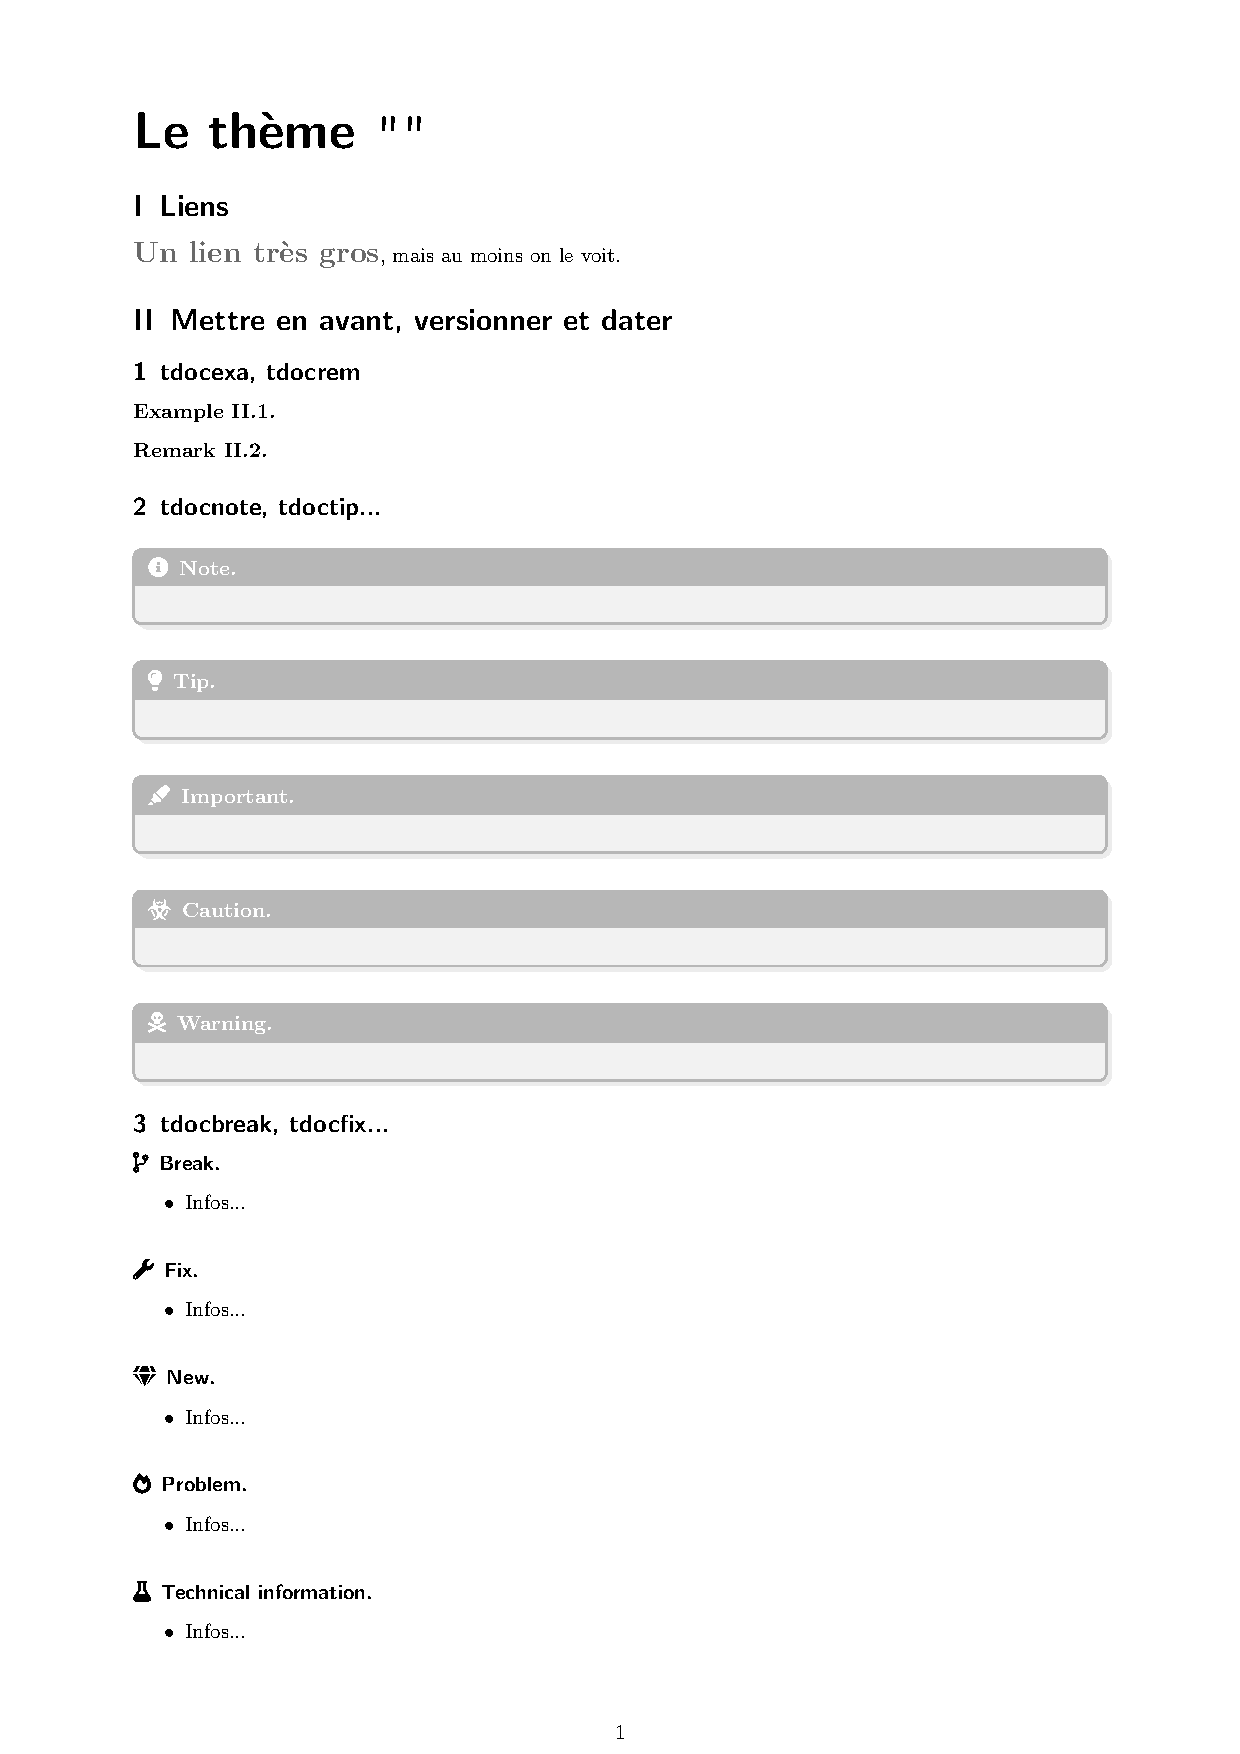
\includepdf{gallery-showcase-bw}

\includepdf{gallery-showcase-color}

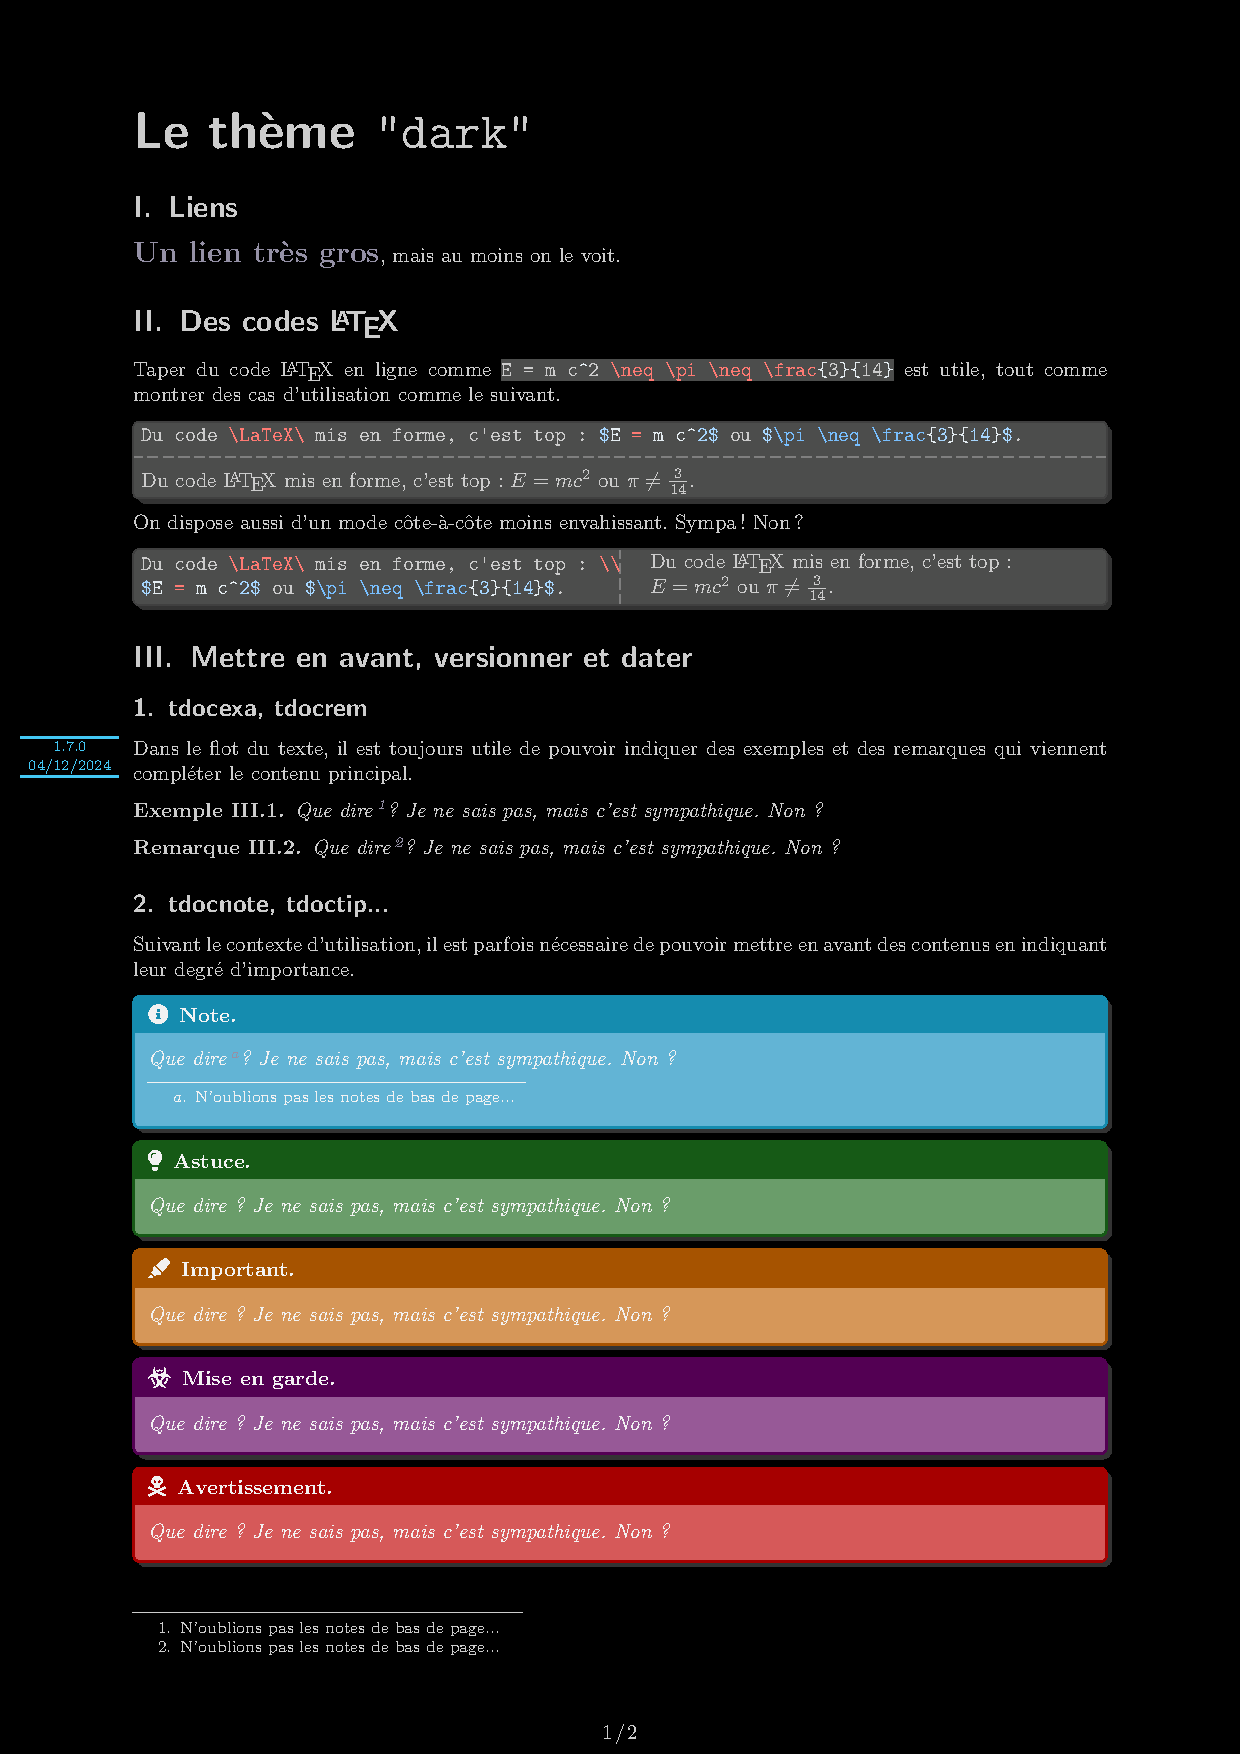
\includepdf{gallery-showcase-dark}

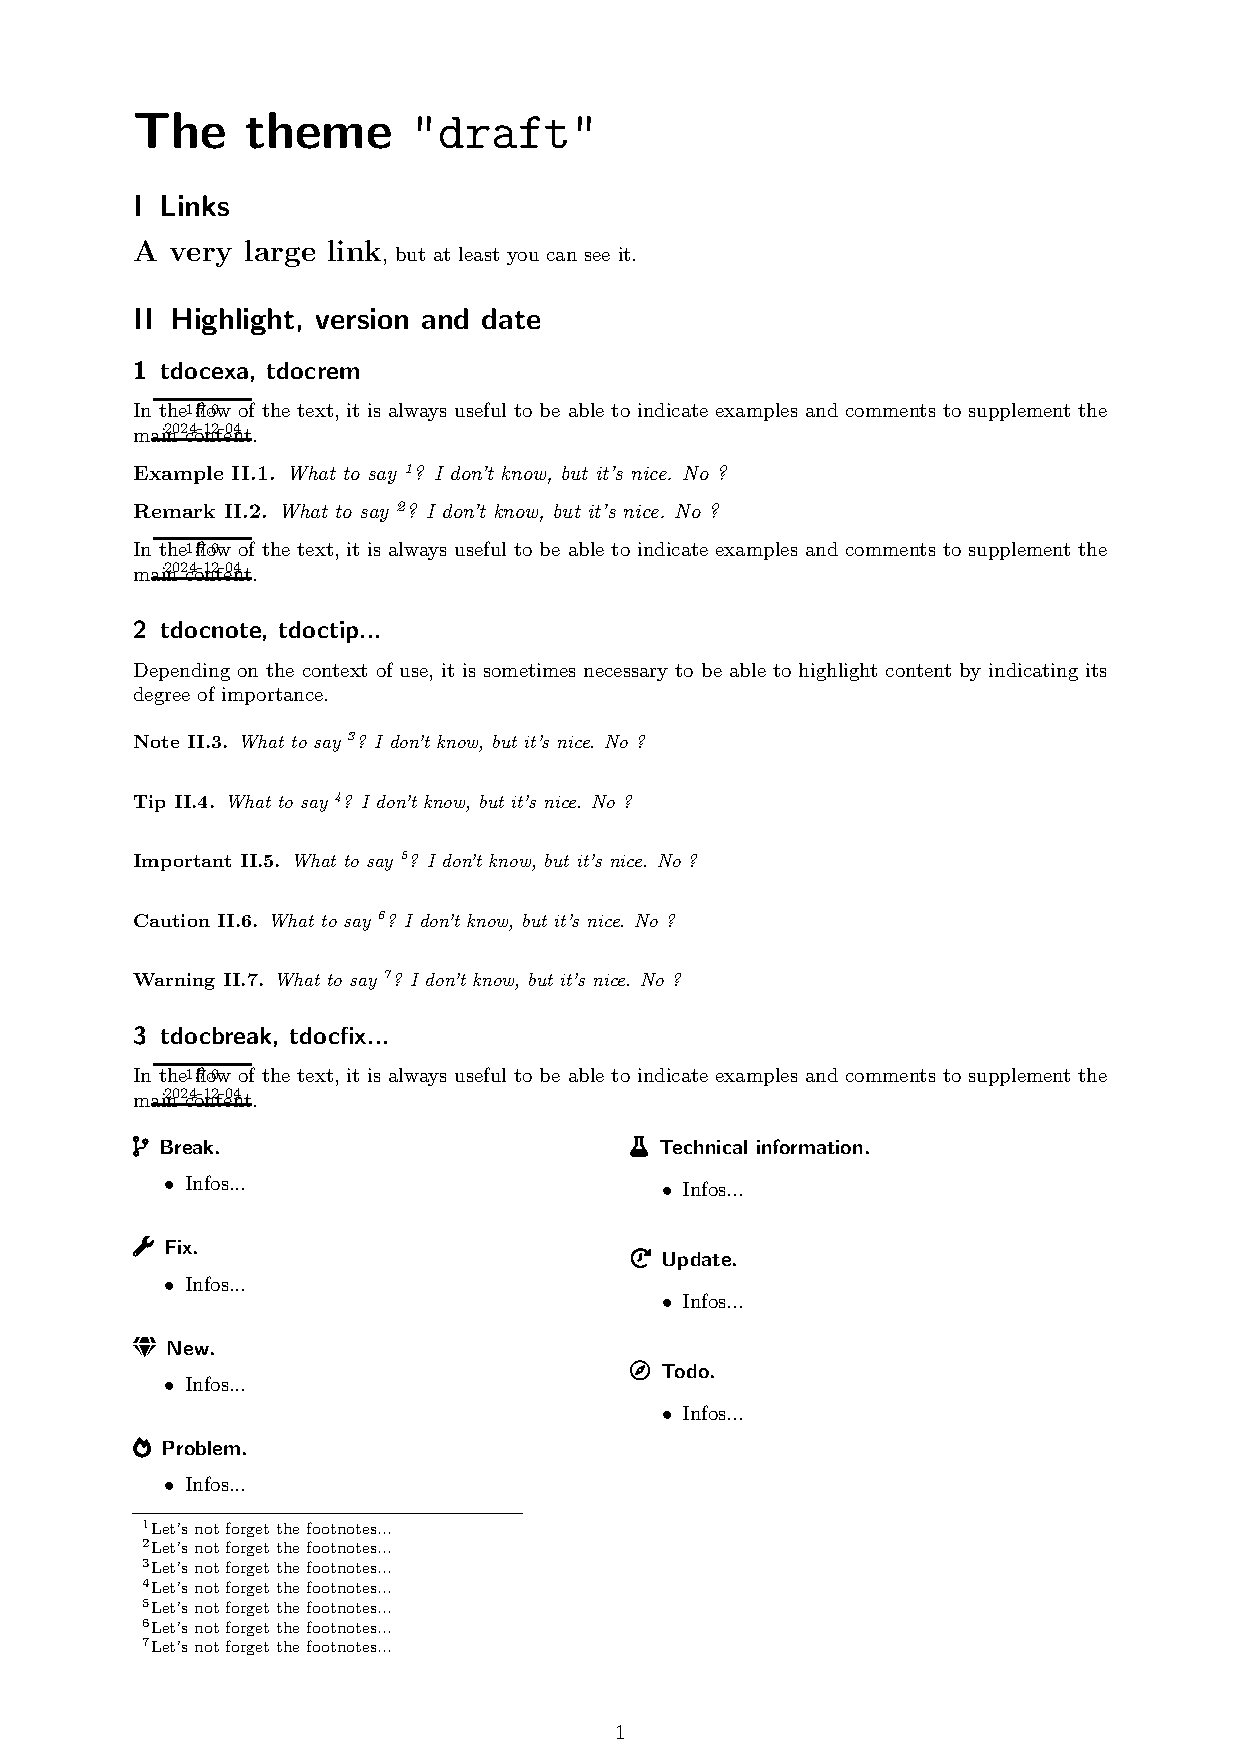
\includepdf{gallery-showcase-draft}

}

% --------------------------- %
% -- AT END DOCUMENT - END -- %
% --------------------------- %

\section{Highlighting content}

\begin{tdocnote}
    The environments presented in this section\,%
    \footnote{
        The formatting comes from the \tdocpack{keytheorems} package.
    }
    add a short title indicating the type of information provided.
    This short text will always be translated into the language detected by the \thisproj\ class.
\end{tdocnote}


\subsection{Content in the reading flow}


\begin{tdocimp}
    All the environments presented in this section share the same counter, which will be reset to zero as soon \tdoclatexin|\section| is used.
\end{tdocimp}


\subsubsection{Examples}

Numbered examples are indicated via \tdocenv{tdocexa}, which offers an optional argument for adding a small title.
Here are two possible uses.

\tdoclatexinput<\tdoctcb{sbs}>{examples-admonitions-exa.tex}


\begin{tdoctip}
    It can sometimes be useful to return to the line at the start of the content. The code below shows how to proceed (this trick also applies to the \verb#tdocrem# environment presented next). Note in passing that the numbering follows that of the previous example as desired.
\end{tdoctip}

\tdoclatexinput<\tdoctcb{sbs}>{examples-admonitions-exa-leavevmode.tex}


% \subsection{Content in the reading flow}

\subsubsection{Some remarks}

Everything happens via \tdocenv{tdocrem}, which works identically to the \tdocenv*{tdocexa} environment, as shown in the following example.

\tdoclatexinput<\tdoctcb{sbs}>{examples-admonitions-rmk.tex}


\subsection{Flashy content}
\label{tutodoc-admonitions}

\begin{tdocnote}
    The formatting proposed here is the default one, but others are possible by changing the theme: see the gallery of use cases in the appendix page \pageref{tutodoc-theme-gallery}.
    As for the icons, they are obtained via the \tdocpack{fontawesome5} package, and the \tdocmacro{tdocicon} macro which manages the spacing relatively to the text.%
    \footnote{
        For example,
        \tdoclatexin|\fbox{tdocicon{faBed}{Fatigued}}|
        produces
        \fbox{\tdocicon{\faBed}{Fatigued}}\,.
    }
\end{tdocnote}


\subsubsection{A tip}

The \tdocenv*{tdoctip} environment is used to give tips. Here's how to use it.

\tdoclatexinput<\tdoctcb{sbs}, bottom = 3pt, top = 3pt>{examples-admonitions-tip.tex}


\smallskip


\begin{tdoctip}
    Sometimes, highlighted content can be reduced to a list. In this case, the formatting can be improved as follows where we use the \tdoclatexin{wide} option from the \tdocpack{enumitem} package imported by this documentation.

    \tdoclatexinput<\tdoctcb{sbs}, bottom = 3pt, top = 3pt>{examples-admonitions-leavevmode-items.tex}
\end{tdoctip}


\foreach \sectitle/\desc/\filename in {
    {Informative note}/%<-- Translate me!
    {The \tdocenv*{tdocnote} environment is used to highlight useful information. Here's how to use it.}/%<-- Translate me!
    note,
    %
    {Something important}/%<-- Translate me!
    {The \tdocenv*{tdocimp} environment is used to indicate something important but harmless.}/%<-- Translate me!
    important,
    %
    {Caution about a delicate point}/%<-- Translate me!
    {The \tdocenv*{tdoccaut} environment is used to indicate a delicate point to the user. Here's how to use it.}/% <-- Translate me!
    caution,
    %
    {Warning of danger}/%<-- Translate me!
    {The \tdocenv*{tdocwarn} environment is used to warn the user of a trap to avoid. Here's how to use it.}/%<-- Translate me!
    warn%
} {
    \subsubsection{\sectitle}

    \desc

    \tdoclatexinput<\tdoctcb{sbs}, bottom = 3pt, top = 3pt>{examples-admonitions-\filename.tex}
}


\section{Specify packages, classes, macros or environments}

Here's what you can type semantically.


\begin{tdoclatex}<\tdoctcb{sbs}>
\tdoccls{myclass} is for...    \\
\tdocpack{mypackage} is for... \\
\tdocmacro{onemacro} is for... \\
\tdocenv{env} produces...      \\
Just \tdocenv*{env}...
\end{tdoclatex}


\begin{tdocrem}
    Unlike \tdocmacro{tdoclatexin}, the \tdocmacro{tdocmacro}, \tdocmacro{tdocenv} and \tdocmacro{tdocenv*} macros don't color the text they produce.
    In addition, \tdoclatexin{\tdocenv{monenv}} produces \tdocenv{monenv} with breakable spaces to allow line breaks if required.
\end{tdocrem}


\section{Origin of a prefix or suffix}

To explain the names chosen, there is nothing like indicating and explaining the short prefixes and suffixes used. This is easily done as follows.


\begin{tdoclatex}<\tdoctcb{sbs}>
\tdocpre{sup} relates to...      \\
\tdocprewhy{sup.erbe} means...   \\
\emph{\tdocprewhy{sup.er} for...}
\end{tdoclatex}


\begin{tdocrem}
    The choice of a full stop to split a word allows words with a hyphen to be used, as in \tdoclatexin+\tdocprewhy{bric.k-breaker}+ which gives \tdocprewhy{bric.k-breaker}.
\end{tdocrem}


\section{A real-life rendering}
\label{tutodoc-showcase}

It is sometimes useful to render code directly in the documentation. This requires the rendering to be dissociable from the explanatory text.



\subsection{A minimalist rendering by default}

\begin{tdocexa}
    It can be useful to show a real rendering directly in a document.%
    \footnote{
        Typically when making a demo.
    }
    This is typed via the environment \tdocenv*{tdocshowcase} as follows.

    \tdoclatexshow[explain = {This results in the following rendering, which is a combination of low vertical spacing and simple import.}]{examples-showcase-default.tex}
\end{tdocexa}


\begin{tdocrem}
    The section \ref{tutodoc-listing-latexshow} on page \pageref{tutodoc-listing-latexshow} explains how to obtain, via the macro \tdocmacro{tdoclatexshow}, a code followed by its actual rendering as in the previous example.
\end{tdocrem}


\begin{tdocwarn}
    With the default settings, if the code to be formatted begins with an opening bracket, we must use one of the following tricks.

    \tdoclatexshow[explain = {This will produce the following.}]{examples-showcase-hook.tex}
\end{tdocwarn}


\subsection{With framing lines}

To make the formatted \LaTeX\ code more visible, you can use the \tdoclatexin{rule} style, as in the following examples.


\begin{tdocexa}
	The option \tdoclatexin{style = rule} provides the following where the automatically added texts will adapt to the language found by \thisproj.

	\begin{tdocshowcase}[style = rule]
    Bla, bla, bla, bla, bla, bla, bla, bla, bla, bla, bla, bla, bla...
\end{tdocshowcase}

\end{tdocexa}


\begin{tdocexa}[Editable text and colours]
	You can easily obtain the following horror.

	\begin{tdocshowcase}[style      = rule,
                     col-stripe = red,
                     col-text   = orange!75!black,
                     before     = Mon début,
                     after      = Ma fin à moi]
    Bla, bla, bla, bla, bla, bla, bla, bla, bla, bla, bla, bla, bla...
\end{tdocshowcase}


	Here's the code that was used.%
	\footnote{
		The next section will justify the a priori strange choice of \tdoclatexin{col-stripe} instead of \tdoclatexin{col-rule}\,.
	}

	\tdoclatexinput<\tdoctcb{code}>{examples-showcase-rule-custom.tex}
\end{tdocexa}


\begin{tdocnote}
    In the previous example, the text uses the proposed darkened orange. However, the red is used as a base to obtain the colors used for the framing lines: the transformations used depend on the theme chosen.%
    \footnote{
        For example, the themes \tdoclatexin{bw} and \tdoclatexin{draft} ignore the key \tdoclatexin{col-stripe}!
    }
    You should also be aware that behind the scenes, the macro \tdocmacro{tdocruler} is used, it works as follows.

    \begin{tdoclatex}<\tdoctcb{std}>
\tdocruler[red]{A decorated pseudo-title}
    \end{tdoclatex}
\end{tdocnote}


\subsection{With colored stripe}

There are situations where you need to be able to clearly identify an example of formatted \LaTeX\ code. This can be done, as the following examples show.%
\footnote{
    Behind the scenes, the strips are created effortlessly using the \tdocpack{clrstrip} package.
}


\begin{tdocexa}
	The \tdoclatexin{style = stripe} option provides the following.

	\begin{tdocshowcase}[style = stripe]
    Bla, bla, bla, bla, bla, bla, bla, bla, bla, bla, bla, bla, bla...
\end{tdocshowcase}

\end{tdocexa}


\begin{tdocexa}[Editable text and colors]
	You can easily produce a beautiful horror like the one below.

	\begin{tdocshowcase}[style      = stripe,
                     col-stripe = green,
                     col-text   = purple,
                     before     = Mon début,
                     after      = Ma fin à moi]
    Bla, bla, bla, bla, bla, bla, bla, bla, bla, bla, bla, bla, bla...
\end{tdocshowcase}

	
	Here's the code that was used.%
	\footnote{
		Now we understand why we chose \tdoclatexin{col-stripe} instead of \tdoclatexin{col-rule}\,.
	}

	\tdoclatexinput<\tdoctcb{code}>{examples-showcase-stripe-custom.tex}
\end{tdocexa}


\subsection{By importing the \LaTeX\ code}

To obtain renderings by importing the code from an external file, instead of typing it, simply use the macro \tdocmacro{tdocshowcaseinput} whose option uses the same syntax as that of the environment \tdocenv*{tdocshowcase}, and the mandatory argument corresponds to the path of the file. Here are some examples of use.


\foreach \exatitle/\style in {
    {Standard use}/%            <-- Translate me!
    	{default},
    {With framing lines}/% <-- Translate me!
    	{rule},
    {A colored stripe}/%         <-- Translate me!
    	{stripe}%
}{
	\begin{tdocexa}[\exatitle]
		\leavevmode
		\tdoclatexinput<\tdoctcb{code}>{examples-showcase-input-\style.tex}

		This gives:

		\smallskip

		\input{examples-showcase-input-\style.tex}
	\end{tdocexa}
}


\section{Use cases in \LaTeX}
\label{tutodoc-listing-latex}

Documenting a package, or class, is best done through use cases showing both the code and the corresponding result.%
\footnote{
    Code is formatted using the \tdocpack{minted} and \tdocpack{tcolorbox} packages.
}


\subsection{\tdocquote{Inline} codes}
\label{tutodoc-listing-latex-inline}

\begin{tdocexa}[Standard use]
    The \tdocmacro{tdoclatexin} macro\,%
    \footnote{
        The name of the macro \tdocmacro{tdoclatexin} comes from \tdocquote{\tdocprewhy{in.line} \LaTeX}\,.
    }
    can be used to type code in line in a similar way to \tdocmacro{verb}, or as a standard macro (see the handling of braces in the latter case below).
    Here are some examples of use.%
    \footnote{
    	A background color is deliberately used to subtly highlight the \tdoclatexin{\LaTeX} codes.
    }

    \begin{tdoclatex}<\tdoctcb{sbs}>
1: \tdoclatexin|$a^b = c$|               \\
2: \tdoclatexin+\tdoclatexin|$a^b = c$|+ \\
3: \tdoclatexin{\tdoclatexin{$a^b = c$}}
	\end{tdoclatex}
\end{tdocexa}


\begin{tdocexa}[Possible options]
    As the \tdocmacro{tdoclatexin} macro is based on \tdocpack{minted}, you can use all the options taken into account by \tdocpack{minted}.
    Here are some examples.

    \begin{tdoclatex}<\tdoctcb{sbs}>
1: \tdoclatexin[style = bw]{$a^b = c$} \\
2: \tdoclatexin[style = igor,
                showspaces]{$a^b = c$}
	\end{tdoclatex}
\end{tdocexa}


\begin{tdocnote}
	The \tdocmacro{tdoclatexin} macro can be used in a footnote as shown below.%
    \footnote{
        \tdoclatexin+$minted = TOP$+ has been typed \tdoclatexin|\tdoclatexin+$minted = TOP$+| in this footnote.
    }
\end{tdocnote}


\subsection{Directly typed codes}

\begin{tdocexa}[Side by side]
    Displaying a code and its rendering side by side is done as follows where the macro \tdocmacro{tdoctcb} allows you to just type \tdoclatexin{tdoctcb{sbs}} instead of \tdoclatexin{listing side text} (\tdoclatexin#sbs# is for \tdocquote{\tdocprewhy{s.ide} \tdocprewhy{b.y} \tdocprewhy{s.ide}}, while \tdoclatexin#tcb# is the standard abbreviation for \texttt{tcolorbox}). Note the use of rafters, not square brackets (more on this later).

    \tdoclatexshow{examples-listing-latex-ABC.tex}
\end{tdocexa}


\begin{tdocexa}[Following]
    \tdocenv{tdoclatex} produces the following result (this default setting is also obtained by using \tdoclatexin#\tdoctcb{std}#).%
    \footnote{
        \tdoclatexin{std} refers to the \tdocquote{standard} behaviour of \tdocpack{tcolorbox} in relation to the \tdocpack{minted} library.
    }

    \begin{tdoclatex}
$A = B + C$
    \end{tdoclatex}
\end{tdocexa}


\begin{tdocexa}[Just the code]
    Via \tdoclatexin#\tdoctcb{code}#, we'll just get the code as below.

    \begin{tdoclatex}<\tdoctcb{code}>
$A = B + C$
    \end{tdoclatex}
\end{tdocexa}


\begin{tdocexa}[Customise]
	The \tdocenv*{tdoclatex} environment accepts two types of optional argument.
	%
	\begin{enumerate}
		\item Between classic square brackets, you can use any option taken into account by \tdocpack{minted}.

		\item Between rafters, you can use any option managed by the environments obtained via \tdocpack{tcolorbox}.
	\end{enumerate}

	For example, the following modifications can be made if required.%
	\footnote{
		This documentation uses the options between rafters to obtain correct rendering of code producing shaded frames: see the section \ref{tutodoc-admonitions} on page \pageref{tutodoc-admonitions}.
	}

    \tdoclatexshow{examples-listing-latex-ABC-custom.tex}
\end{tdocexa}

\medskip

\begin{tdocwarn}
    To obtain the default formatting for a code beginning with a bracket or a rafter, you'll need to do a bit of fiddling, as shown below.
    \tdoclatexshow{examples-listing-latex-strange.tex}

    \smallskip

    Another method is to use the \tdocmacro{string} primitive, as shown below.
    \tdoclatexshow{examples-listing-latex-strange-bis.tex}
\end{tdocwarn}


\subsection{Imported codes}

For the following codes, consider a file with the relative path \verb+examples-listing-xyz.tex+, and with the following contents.

\tdoclatexinput<\tdoctcb{code}>{examples-listing-latex-xyz.tex}

\medskip

The \tdocmacro{tdoclatexinput} macro, shown below, expects the path of a file and offers the same system of options between square brackets, or rafters, as the environment \tdocenv*{tdoclatex}.

\foreach \title/\extra/\fname in {%
	{Side by side}/%
		{}/%
		sbs,
	{Following}/%
		{, which also corresponds to the option \tdoclatexin{\tdoctcb{std}}\,}/%
		std,%
	{Only the code}/%
		{}/%
		code,%
	{Customise}/%
		{}/%
		perso%
}{
	\begin{tdocexa}[\title]
    	\leavevmode
		\tdoclatexshow[explain=This produces the following formatting\extra.]{examples-listing-latex-latexinput-option-\fname.tex}
	\end{tdocexa}
}



\subsection{Imported codes put into practice}
\label{tutodoc-listing-latexshow}

\begin{tdocnote}
    The default texts take into account the language detected by \thisproj.
\end{tdocnote}


\begin{tdocexa}[Showcase]
    The following comes from \tdoclatexin+\tdoclatexshow{examples-listing-xyz.tex}+.

    \smallskip

    \tdoclatexshow{examples-listing-latex-xyz.tex}
\end{tdocexa}


\begin{tdocexa}[Changing the explanatory text]
    Using the key \tdoclatexin|explain|, you can use a custom text. Thus, \tdoclatexin|\tdoclatexshow[explain = Here is the rendering.]{examples-listing-xyz.tex}| will give the following.

    \smallskip

    \tdoclatexshow[explain = Here is the rendering.]{examples-listing-latex-xyz.tex}
\end{tdocexa}


\begin{tdocexa}[The options available]
    In addition to the explanatory text, it is also possible to use all the options of \tdocenv*{tdocshowcase} environment, see \ref{tutodoc-showcase} on page \pageref{tutodoc-showcase}.
    Here is an example to illustrate this.

    \medskip

    \tdoclatexinput<\tdoctcb{code}>{examples-listing-latex-latexshow-options.tex}

    \smallskip

    This will produce the following.

    \smallskip

    \tdoclatexshow[explain   = Ce qui vient est coloré...,
               before    = Rendu ci-après.,
               after     = Rendu fini.,
               col-stripe = orange,
               col-text   = blue!70!black]
               {examples-listing-latex-xyz.tex}

\end{tdocexa}


\section{Presenting computer code}

Some packages offer functions that require to code a little in \lua.%.
\footnote{
	For mathematics, these include \tdocpack{luacas} and \tdocpack{tkz-elements}.
}
For these projects, the documentation must be able to present lines of code; this is why \thisproj\ makes it easy to do this, and much more.%
\footnote{
    As code formatting is done via the packages \tdocpack{minted} and \tdocpack{tcolorbox}, the macros and environments presented in this section allow code to be formatted in all the languages supported by \pygmentsREF, a \python\ project used behind the scenes by \tdocpack{minted}.
}


\begin{tdocimp}
	The tools in this section can also be used to present \LaTeX code, but they should not be used for simple use cases, as the macros and environments presented next are for studying code, not just for using it: see the section \ref{tutodoc-listing-latex} on page \pageref{tutodoc-listing-latex} to use the right tools for formatting \LaTeX\ use cases.
\end{tdocimp}



\subsection{\tdocquote{Inline} codes}

The \tdocmacro{tdoccodein}\,%
\footnote{
	The name of the macro \tdocmacro{tdoccodein} comes from \tdocquote{\tdocprewhy{in.line} \tdocpre{code}}\,.
}
macro expects two arguments: the \ordinalnum{1} indicates the programming language, and the \ordinalnum{2} gives the code to be formatted.
It is possible to use an option identical to that proposed by \tdocmacro{tdoclatexin}: see the section \ref{tutodoc-listing-latex-inline} on page \pageref{tutodoc-listing-latex-inline}.
Here are some possible use cases.%
\footnote{
    A background color is used to subtly highlight the formatted codes. For example, typing \tdoclatexin{\tdoccodein{py}{funny = "ah"*3}} will produce \tdoccodein{py}{funny = "ah"*3}\,.
}

\begin{tdoclatex}
1: \tdoccodein{py}{print("OK" if i = 0 else "KO")}             \\
2: \tdoccodein[style = bw]{py}{print("OK" if i = 0 else "KO")} \\
3: \tdoccodein[style = igor, showspaces]%
              {py}{print("OK" if i = 0 else "KO")}
\end{tdoclatex}

\medskip

\begin{tdocnote}
	The page \url{https://pygments.org/languages} contains a complete list of supported languages with their short names. For example, it is possible to format \brainfuck\ code like this obscure sequence \tdoccodein{bf}{++++++++++[>+++++++>++++++++++>+++>+<<<<-]>++.>+.+++++++..+++.} which displays \tdoccodein{text}{Hello}\,.
\end{tdocnote}



\subsection{Codes typed directly}

Code can be typed directly into a document via \tdocenv{tdoccode} which expects an argument indicating the programming language, and any options between parenthesis and/or square brackets identical to those proposed by \tdocenv{tdoclatex}: see the section \ref{tutodoc-listing-latex} on page \pageref{tutodoc-listing-latex}.%
\footnote{
	Note that the coloring of the \LaTeX\ codes is lexically correct, but semantically wrong.
}


% Strings "..." in the source codes must also be translated.
\foreach \title/\lang in {%
	{Standard feature}/%
		perl,%
	{One-off rendering customization}/%
		lua%
}{
    \begin{tdocexa}[\title]
    	\leavevmode
    	\tdoclatexshow{examples-listing-full-hello-you-\lang}
    \end{tdocexa}
}


\subsection{Imported codes}

The \tdoclatexin{tdoccodeinput} macro expects the language and path of a file to be formatted, and possibly options similar to those offered by the \tdocenv*{tdoccode} environment.


% Strings "..." in the source codes must also be translated.
\foreach \title/\lang in {%
	{Standard features}/%
		hs,%
	{Customize rendering on occasion}/%
		tex%
}{
    \begin{tdocexa}[\title]
    	\leavevmode
    	\tdoclatexinput<\tdoctcb{code}>{examples-listing-full-input-hello-you-\lang}

		This gives:

		\documentclass[10pt, a4paper]{main}

\usepackage[utf8]{inputenc}
\usepackage[T1]{fontenc}

\usepackage[french]{babel, varioref}

\usepackage{enumitem}
\frenchsetup{StandardItemLabels=true}

\usepackage{tabularray}

\usepackage[lang = french]{tutodoc}


\usepackage{../admonitions/admonitions.cls}
\usepackage{../inenglish/inenglish.cls}
\usepackage{../listing/listing.cls}
\usepackage{../macroenv/macroenv.cls}


\begin{document}

\section{Quelle langue est utilisée par la classe \thisproj\ ?}

Cette documentation charge le package \tdocpack{babel} via \tdocinlatex|\usepackage[french]{babel}|\,.
Dès lors, la classe \thisproj\ repère \tdocinlatex|fr| comme langue principale utilisée par \tdocpack{babel}.%
\footnote{
	Techniquement, on utilise \tdocinlatex|\BCPdata{language}| qui renvoie une langue au format court.
}
Comme cette langue fait partie de la liste des langues prises en compte, voir ci-dessous, la classe \thisproj\ produira les effets attendus.
% Do not touch the following placeholder.
<<ALL-LANGS>>


\begin{tdoccaut}
	Si le choix de la langue principale n'est pas faite dans le préambule, le mécanisme employé échouera avec des effets de bord non voulus (voir l'avertissement qui suit).
\end{tdoccaut}


\begin{tdocwarn}
    Lorsqu'une langue n'est pas prise en compte par \thisproj, un message d'avertissement est émis, et l'anglais est alors choisi comme langue vis-à-vis de \thisproj.
\end{tdocwarn}


\begin{tdocnote}
    Le mécanisme utilisé devrait être compatible avec le package \tdocpack{polyglossia}.
\end{tdocnote}

\end{document}

    \end{tdocexa}
}


\section{Indicate changes}
\label{tutodoc-changes}

To make it easier to monitor a project, it is essential to provide a history indicating the changes made when a new version is published.



\subsection{When?}
\label{tutodoc-changes-when}

You can date and/or version something.


\begin{tdocexa}[Dating new features]
    The \tdocmacro{tdocdate} macro is used to indicate a date in the margin, as in the following example.

    \tdoclatexshow{examples-version-n-change-dating.tex}
\end{tdocexa}


\begin{tdocexa}[Versioning new features, possibly with a date]
    Associating a version number with a new feature is done using the \tdocmacro{tdocversion} macro, with the color and date being optional arguments.

    \tdoclatexshow{examples-version-n-change-versioning.tex}
\end{tdocexa}


\begin{tdocexa}[Caution with paragraph titles]
	The following example shows that a date and/or version must be placed just after a paragraph title, and not before it.

	\tdoclatexshow{examples-version-n-change-para-title.tex}
\end{tdocexa}


\begin{tdocexa}[Adjust vertical shift]
	If required, you can modify the vertical offset used to place dates and versions in the margin, the default value being $(-8\,\mathit{pt})$.

	\tdoclatexshow{examples-version-n-change-manual-setting.tex}
\end{tdocexa}


\begin{tdocimp}
    \begin{enumerate}[wide]
        \item The \tdocmacro{tdocdate} and \tdocmacro{tdocversion} macros require two compilations.

        \item The final rendering of the dates takes into account the language detected by \thisproj{}: for example, if French is selected, the dates will be displayed in the format \texttt{DD/MM/YYYY}.
    \end{enumerate}
\end{tdocimp}


\begin{tdoccaut}
    Only the use of the digital format \tdoclatexin+YYYY-MM-DD+ is verified,%
    \footnote{
        Technically, checking the validity of a date using \LaTeX3 presents no difficulty.
    }
    and this is a choice! Why? Quite simply because dating and versioning explanations should be done semi-automatically to avoid any human bugs.
\end{tdoccaut}


\subsection{What's new?}

\thisproj\ offers the macro \tdocmacro{tdocstartproj} and different environments to indicate quickly and clearly what has been done during the changes made, or to come.%
\footnote{
    The user doesn't need all the technical details.
}


\begin{tdocnote}
    For icons, see the note at the beginning of the section \ref{tutodoc-admonitions} on page \pageref{tutodoc-admonitions}.
\end{tdocnote}


\subsubsection{Sobriety first}

\foreach \exatitle/\filename in {
% Standard.
    {Just for the very first version}/%<-- Translate me!
        first,
    {For new features}/% <-- Translate me!
        new,
    {For updates}/% <-- Translate me!
        update,
    {For breaks}/% <-- Translate me!
        break,
    {For problems}/% <-- Translate me!
        pb,
    {For fixes}/% <-- Translate me!
        fix,
    {Roadmap}/% <-- Translate me!
        todo,
    {Technical information}/% <-- Translate me!
        tech,
% Customized.
    {Selectable themes with an icon}/% <-- Translate me!
        user-choice-icon,
    {Selectable themes without icons}/%<-- Translate me!
        user-choice%
} {
    \begin{tdocexa}[\exatitle]
        \leavevmode

        \tdoclatexinput<\tdoctcb{sbs}>{examples-version-n-change-chges-\filename.tex}
    \end{tdocexa}
}


\subsubsection{Color if necessary}

It may be useful to highlight some changes: this can only be done by modifying the content color.

\foreach \exatitle/\filename in {
    {A flashy first version}/%<-- Translate me!
        first,
    {Outstanding fixes}/% <-- Translate me!
        fix%
} {
    \begin{tdocexa}[\exatitle]
        \leavevmode

        \tdoclatexinput<\tdoctcb{sbs}>{examples-version-n-change-color-chges-\filename.tex}
    \end{tdocexa}
}


\subsection{The what and the when}

The optional keys \tdoclatexin{col-chges}\,, \tdoclatexin{date} and \tdoclatexin{version} allow to date and/or version a change of a particular type.
Here are some examples of use.

\tdoclatexshow{examples-version-n-change-what-n-when.tex}


\section{Ornament}

Let's finish this documentation with a small formatting tool that can be very useful.


\begin{tdoclatex}<\tdoctcb{sbs}>
Bla, bla, bla...

\tdocsep % Practical for demarcation.

This works with enumerations.

\begin{itemize}
    \item Focus.
\end{itemize}

\tdocsep % Uniform behaviour.

Ble, ble, ble...
\end{tdoclatex}


\section{Contribute}

\begin{tdocnote}
    \textbf{You don't need to be a coder to take part in translations}, including those that are useful for the running of \thisproj.
\end{tdocnote}


%\section{Contribute}

\subsection{Complete the translations}

\begin{tdocnote}
    The author of \thisproj\ manages the French and English versions of the translations.
\end{tdocnote}


\begin{tdoccaut}
    Although we're going to explain how to translate the documentation, it doesn't seem relevant to do so, as English should suffice these days.%
    \footnote{
      The existence of a French version is simply a consequence of the native language of the author of \thisproj.
    }
\end{tdoccaut}


\begin{figure}[ht]
    \centering
    \contribtranslatedirtree\
    \caption{Simplified view of the translation folder}
    \label{tutodoc-contrib-translate-dir}
\end{figure}


The translations are roughly organized as in figure \ref{tutodoc-contrib-translate-dir} where just the important folders for the translations have been \tdocquote{opened}\,.%
\footnote{
    This was the organization on October 5, 2024.
}
\textbf{A little further down, the section \ref{tutodoc-contrib-translate} explains how to add new translations}.


\subsubsection{The \texttt{fr} and \texttt{en} folders}

These two folders, managed by the author of \thisproj, have the same organization; they contain files that are easy to translate even if you're not a coder.


\subsubsection{The \texttt{changes} folder}

This folder is a communication tool where important changes are indicated without dwelling on minor modifications specific to one or more translations.


\subsubsection{The \texttt{status} folder}

This folder is used to keep track of translations from the project's point of view. Everything is done via well-commented \verb#YAML# files, readable by a non-coder.


\subsubsection{The \texttt{README.md} and \texttt{LICENSE.txt} files}

The \texttt{LICENSE.txt} file is aptly named, while the \texttt{README.md} file takes up in English the important points of what is said in this section about new translations.


\subsubsection{New translations}
\label{tutodoc-contrib-translate}

\begin{tdocimp}
    The \verb#api# folder contains translations relating to the functionalities of \thisproj.
    Here you'll find \verb#TXT# files for editing with a text or code editor, but not with a document processor.
    The content of these files uses commented lines in English to explain what \thisproj\ will do; these lines begin with \verb#//#\,. Here's an extract from such a file, where translations are made after each \,$=$\ sign, without touching the preceding, as this initial piece is used internally by the \thisproj\ code.

    \tdocsep
    \vspace{-10pt}
    \begin{verbatim}
    // #1: year  in format YYYY like 2023.
    // #2: month in format MM   like 04.
    // #3: day   in format DD   like 29.
    date = #1-#2-#3

    // #1: the idea is to produce one text like
    //     "this word means #1 in English".
    in_EN = #1 in english\end{verbatim}
\end{tdocimp}


\begin{tdocnote}
    The \verb#doc# folder is reserved for documentation. It contains \verb#TEX# files that can be compiled directly for real-time validation of translations.
\end{tdocnote}


\begin{tdocwarn}
    Only start from one of the \verb#fr# and \verb#en# folders, as these are the responsibility of the \thisproj\ author.
\end{tdocwarn}


\medskip


\emph{\textbf{Let's say you want to add support for Italian from files written in English.}}%
\footnote{
    As mentioned above, there is no real need for the \texttt{doc} folder.
}


\paragraph{Method 1 : use of \git.}

\begin{enumerate}
      \item Recover the entire project folder via \thisrepo\,.
    Do not use the \verb#main# branch, which is used to freeze the latest stable versions of projects in the single \thismonorepo\ repository,.

      \item In the \verb#tutodoc/contrib/translate# folder, create an \verb#it# copy of the \verb#en# folder, with the short name of the language documented in
      \href{https://en.wikipedia.org/wiki/IETF_language_tag#List_of_common_primary_language_subtags}%
           {the page \tdocquote{IIETF language tag}}
      from \texttt{Wikipedia}.

      \item Once the translation is complete in the \verb#it# folder, share it via \thisrepo\ using a classic \verb#git push#\,.
\end{enumerate}


\paragraph{Method 2 : communicate by e-mail.}

\begin{enumerate}
      \item By e-mail with the \mailsubject{en FOR italian}, request a version of the English translations (note the use of the English name for the new language).
    Be sure to respect the subject of the e-mail, as the author of \thisproj\ automates the pre-processing of this type of e-mail.

      \item You will receive a folder named \verb#italian# containing the English version of the latest translations.
    This folder will be the place for your contribution.

      \item Once the translation is complete, you will need to compress your \verb#italian# file in \verb#zip# or \verb#rar# format before sending it by e-mail with the \mailsubject{italian}\,.
\end{enumerate}


%\section{Contribute}

\subsection{Improving the source code}

\begin{tdocimp}
    If you want to participate to \thisproj\,, you'll need to use the \LaTeX3 programming paradigm.
\end{tdocimp}


Participation as a coder is made via the repository \thisrepo\ corresponding to the \verb#tutodoc# development branch.


\begin{tdoccaut}
Do not use the \verb#main# branch, which is used to freeze the latest stable versions of projects in the mono repository \thismonorepo.
\end{tdoccaut}


\section{History}

\small

\begin{tdocfix}[version = 1.7.1, date = 2024-12-18]
	\item Documentation: references to tools to indicate changes have been incorrectly written as characteristics of highlighted colored content.
\end{tdocfix}


\begin{tdocbreak}
	\item The \tdocmacro{tdocenv} macro and its starred version no longer offer an option.
	
	\item \LaTeX\ showcases: the default layout is more sober, and there are options for having just the rulers, or the colored stripe. See just after.
\end{tdocbreak}


\begin{tdocnew}
	\item Formatting of computer codes in addition to those specifically in \LaTeX.
	%
	\begin{enumerate}
		\item Creation of \tdocenv{tdoccode} and \tdocmacro{tdoccodein}.

		\item For macros for inline code, and environments for blocks of code, \tdocpack{minted} options are indicated inside square brackets in the traditional way: \tdoclatexin{[minted options]}\,.

		\item For code block environments, \tdocpack{tcolorbox} options are indicated inside rafters: \tdoclatexin{<tcolorbox options>}\,.

		\item The new macro \tdocmacro{tdoctcb} allows to use shortcuts for regularly used \tdocpack{tcolorbox} styles.
	\end{enumerate}

	\item Documentation: a new section presents tools for formatting computer codes other than those in \LaTeX.
\end{tdocnew}


\begin{tdocupdate}
	\item Sub-sub-sections are numbered in lower case.

	\item Themes.
	%
	\begin{enumerate}
		\item Less space consumed.

		\item Shadows have better coloring.

		\item For all themes except the \tdoclatexin{draft} one, the radius of the arcs of the corners of the frames has changed from \tdoclatexin{.75mm} to \tdoclatexin{.2pt},.

 		\item Use case in \LaTeX: with the theme \tdoclatexin{color}, the background color changes from \tdoclatexin[bgcolor = yellow!4]{yellow!4} to \tdoclatexin{gray!5}.

		\item Latest changes: with the \tdoclatexin{dark} theme, the \tdoclatexin{[Init]} text produced by the \tdocmacro{tdocstartproj} macro uses the same font as the environment titles to indicate changes.
	\end{enumerate}
\end{tdocupdate}

\tdocsep


% ------------------ %


\begin{tdocbreak}[version = 1.7.0, date = 2024-12-04]
	\item Format: the \tdoccls{scrartcl} class replaces the venerable \tdoccls{article}. This implies better placement of the margin notes with the options retained for loading \tdoccls{scrartcl}.

	\item \LaTeX\ code: the macro \tdocmacro{tdocinlatex} has been renamed \tdocmacro{tdoclatexin}.

	\item Color key names will be hyphenated where necessary: this implies the following changes.
	%
	\begin{enumerate}
		\item Indicate the latest changes: the \tdoclatexin{colchges} option of the environments has been renamed \tdoclatexin{col-chges}.

		\item Showcases: for the environment \tdocenv*{tdocshowcase} and the macro \tdocmacro{tdocshowcaseinput}, the \tdoclatexin{colstripe} and  \tdoclatexin{coltext} options have been renamed \tdoclatexin{col-stripe} and \tdoclatexin{col-text}\,.
	\end{enumerate}
\end{tdocbreak}


\begin{tdocfix}
	\item Admonitions: for the \tdocmacro{newkeytheorem} used with the \tdoclatexin{draft} theme, \tdoclatexin{postheadhook = \leavevmode} has been added (this is necessary because the content can naturally be of the list type).
\end{tdocfix}


\begin{tdocnew}
	\item Documentation: addition of a section listing dependencies.

	\item Class options.
	%
	\begin{enumerate}
		\item Options not specific to \thisproj\ are passed on to the class in charge of general formatting.

		\item The \tdoccls{scrartcl} options \tdoclatexin{fontsize} and \tdoclatexin{DIV} can't be used because their values are fixed by \thisproj.
	\end{enumerate}

	\item The macro \tdocmacro{tdocinEN} respects the English linguistic rules.

	\item Indicate the latest changes.
	%
	\begin{enumerate}
		\item Add the environment \tdocenv{tdoctodo}\,.

		\item Each environment has a new option \tdoclatexin{col} for the color of the content indicating changes.
	\end{enumerate}
\end{tdocnew}


\begin{tdocupdate}
	\item \tdoclatexin{draft} theme and changes: the environments for the latest changes stop to use icons.

	\item Documentation: the theme gallery uses a better fake example.
\end{tdocupdate}



\begin{tdoctech}
	\item Simplified organisation of configuration files in the final project.
	%
	\begin{enumerate}
		\item Use of one file per theme with a name like \texttt{tutodoc-*.css.cls}\,.

		\item Locale: use of names like \texttt{tutodoc-*.loc.cls}\,.
	\end{enumerate}
\end{tdoctech}

\tdocsep


% ------------------ %


\begin{tdocnew}[version = 1.6.2, date = 2024-10-30]
	\item The macros \tdocmacro{tdocdate} and \tdocmacro{tdocversion} has a new final optional argument \tdoclatexin{<voffset>} to choose a specific vertical offset.

	\item Better environments to indicate the changes made.
	\begin{enumerate}
        \item The new optional keys \tdoclatexin{col}\,, \tdoclatexin{date} and \tdoclatexin{version} allow to date and version a change of a specific topic.

        \item Use of \tdocmacro{paragraph} for the title.
	\end{enumerate}
\end{tdocnew}


\begin{tdocupdate}
	\item Version and changes: the font of the margin notes will always have a normal shape.

	\item Ornament: use of a \tdoclatexin{\cleaders} to avoid orphean rules at the bottom of a page.
\end{tdocupdate}

\tdocsep


% ------------------ %


\begin{tdoctech}[version = 1.6.1, date = 2024-10-28]
    \item The naming rules of \ctan\ need the use of \trademark{CSS} files named \verb+tutodoc-*.css.cls.sty+\,.
\end{tdoctech}

\tdocsep


% ------------------ %


\begin{tdocbreak}[version = 1.6.0, date = 2024-10-27]
    \item The \tdocenv*{showcase} environment and its descendants: the \tdoclatexin{color} key has been renamed \tdoclatexin{colstripe}.

    \item The macro \tdocmacro{tdoclinkcolor} becomes the color \tdoclatexin{tutodoc@link@color} for internal use.
\end{tdocbreak}


\begin{tdocnew}
    \item The \tdoclatexin{theme} class option allows you to choose different formatting themes.

    \item Change log: addition of the \tdocenv*{tdoctech} environment for technical information.

    \item The \tdocenv*{showcase} environment and its descendants: the \tdoclatexin{coltext} key can also be used to change the text color.

    \item The new functionalities have been documented.
\end{tdocnew}


\begin{tdocupdate}
    \item Change log: the \tdocenv*{tdocupdate} environment uses the icon
    \raisebox{0pt}[0pt][0pt]{\fbox{\reflectbox{\faHistory}}}
    instead of
    \raisebox{0pt}[0pt][0pt]{\fbox{\faMagic}}\,.
\end{tdocupdate}


\begin{tdocfix}
    \item The Spanish translations were not included in the previous version! Don't laugh too loud...
\end{tdocfix}

\tdocsep


% ------------------ %


\begin{tdoctech}[version = 1.5.0, date = 2024-10-19]
    \item Version 3 of \tdocpack{minted} is taken into account.
\end{tdoctech}


\begin{tdocbreak}
    \item The \thisproj\ class replaces the now-defunct \thisproj\ package (for the moment, the young class offers no specific options).

    \item The \tdocmacro{tdocruler} macro is now used via \tdoclatexin{\tdocruler[<color>]{<text>}} (remember that the old syntax was \tdoclatexin{\tdocruler{<text>}{<color>}}).
\end{tdocbreak}


\begin{tdocnew}
    \item The class is usable in Spanish.

    \item The documentation contains a new section explaining how to contribute.
\end{tdocnew}


\begin{tdocfix}
    \item The \tdocmacro{tdocdate} macro did not handle date format and formatting.

    \item Colored frames did not color text after a page break.
\end{tdocfix}

\tdocsep


% ------------------ %


\begin{tdocbreak}[version = 1.4.0, date = 2024-09-28]
    \item The \tdocenv*{tdoccaution} environment has been renamed \tdocenv*{tdoccaut} for simplified input.

    \item Content highlighting: examples and remarks, indicated via the \tdocenv*{tdocexa} and \tdocenv*{tdocrem} environments, are numbered using a common counter.

    \item The unused macro \tdocmacro{tdocxspace} has been deleted.
\end{tdocbreak}


\begin{tdocnew}
    \item Change log: the \tdocmacro{tdocstartproj} macro is used to manage the case of the first public version.

    \item Code factorization: the \tdocmacro{tdocicon} macro is responsible for adding icons in front of text.
\end{tdocnew}


\begin{tdocupdate}
    \item Colors: the \tdocmacro{tdocdarkcolor} and \tdocmacro{tdoclightcolor} macros offer an optional argument.
    \begin{enumerate}
        \item \tdocmacro{tdocdarkcolor}: the amount of color in relation to black can be optionally defined.

        \item \tdocmacro{tdoclightcolor}: the transparency rate can be optionally defined.
    \end{enumerate}

    \item Content highlighting: reduced space around content in colored frames.

    \item Versioning: better vertical spacing thanks to \tdocmacro{vphantom}.
\end{tdocupdate}

\tdocsep


% ------------------ %


\begin{tdocnew}[version = 1.3.1, date = 2024-09-26]
    \item Star version of \tdocmacro{tdocenv} to display only the environment name.
\end{tdocnew}

\tdocsep


% ------------------ %


\begin{tdoctech}[version = 1.3.0, date = 2024-09-25]
    \item Version 3 of \tdocpack{minted} cannot be used for the moment as it contains bugs: see \url{https://github.com/gpoore/minted/issues/401}. We therefore force temporarily the use of version 2 of \tdocpack{minted}.
\end{tdoctech}


\begin{tdocbreak}
    \item The \tdocenv*{tdocimportant} environment has been renamed \tdocenv*{tdocimp} for simplified input.
\end{tdocbreak}


\begin{tdocnew}
    \item Change log: proposed environments use icons.


    \item Content highlighting: colored frames with icons are proposed for the following environments.
    %
    \begin{tasks}[label=\arabic*.](3)
        \task \tdocenv*{tdoccaution}
        \task \tdocenv*{tdocimp}
        \task \tdocenv*{tdocnote}
        \task \tdocenv*{tdoctip}
        \task \tdocenv*{tdocwarn}
    \end{tasks}
\end{tdocnew}

\tdocsep


% ------------------ %


\begin{tdocupdate}[version = 1.2.0-a, date = 2024-08-23]
    \item \tdocmacro{tdocversion}
    \begin{enumerate}
        \item The version number is above the date.

        \item The spacing is better managed when the date is absent.
    \end{enumerate}
\end{tdocupdate}


\begin{tdocfix}
    \item Content highlighting: the French translations of \tdocinEN*{caution} and \tdocinEN*{danger} were incorrect.
\end{tdocfix}

\tdocsep


% ------------------ %


\begin{tdocnew}[version = 1.1.0, date = 2024-01-06]
    \item Change log: two new environments.
    \begin{enumerate}
        \item \tdocenv{tdocbreak} for breaking changes which are not backward compatible.

        \item \tdocenv{tdocprob} for identified problems.
    \end{enumerate}

    \item \tdocmacro{tdoclatexin}: a light yellow is used as the background color.
\end{tdocnew}

\tdocsep


% ------------------ %


\begin{tdocfix}[version = 1.0.1, date = 2023-12-08]
    \item \tdocmacro{tdocenv}: spacing is now correct, even if the \tdocpack{babel} package is not loaded with the French language.

    \item \tdocenv[{[nostripe]}]{tdocshowcase} : page breaks around \tdocquote{framing} lines should be rare from now on.
\end{tdocfix}

\tdocsep


% ------------------ %


\tdocversion{1.0.0}[2023-11-29]
\tdocstartproj{First public version of the project.}

\end{document}
